\documentclass[10pt]{article}

\usepackage{sbc-template}
\usepackage{graphicx}
\usepackage{float}
\usepackage{multicol}
\setlength{\columnsep}{0.7cm}
\graphicspath{{figures/}{./}}
\usepackage{url}
\usepackage[utf8]{inputenc}
\usepackage[brazil]{babel}

\sloppy

\title{Chatbot para Atendimento na Secretaria Acadêmica Utilizando Framework Leve}

\author{Marília Stefenon Rodrigues\inst{1}}

\address{Instituto Federal de Santa Catarina -- Campus Garopaba (IFSC)\\
  Rua Maria Aparecida Barbosa, 153 -- Bairro Campo Duna -- 88.495-000 -- Garopaba -- SC -- Brasil
  \email{marilia.sr@aluno.ifsc.edu.br}
}

\begin{document}

\maketitle

\begin{abstract}
The advancement of computing and artificial intelligence has enabled the
automation of tasks once performed exclusively by humans, such as user
support, typically carried out by chatbots -- virtual agents that
standardize and streamline access to information. At the Federal
Institute of Santa Catarina (IFSC) -- Garopaba Campus, the Academic
Secretary handles demands such as absence justification, early student
release, financial aid, enrollment, course offerings, diplomas and
graduation, mostly through WhatsApp, with no record of service volume or
completion. Given the high demand and limited staff, the sector becomes
overloaded due to the lack of automated responses. This paper presents
the development of a chatbot to support the demands of the Academic
Secretary/Registry, the CERE and the Student Assistance office at the
Garopaba Campus, built with the lightweight Flask framework and a
control panel to log every interaction. Requirements were gathered with the staff member
responsible for the campus secretary, based on the most frequent
WhatsApp requests, together with flow diagrams representing how students
navigate the IFSC website to justify an absence, enroll in a course and
complete enrollment.
\end{abstract}

\begin{resumo}
O avanço da computação e da inteligência artificial, com o
desenvolvimento de máquinas e algoritmos cada vez mais capazes de imitar
o ser humano, tem possibilitado a execução de tarefas antes
exclusivamente humanas, como o atendimento ao usuário -- normalmente
realizado por chatbots, agentes virtuais que padronizam e facilitam o
acesso à informação, podendo inclusive executar tarefas mais complexas
conforme a finalidade. No IFSC -- Câmpus Garopaba, a Secretaria
Acadêmica é responsável por diversas demandas dos alunos e da comunidade
em geral, como justificativa de ausência escolar, saída antecipada,
auxílio financeiro, matrícula, cursos ofertados, diplomas e formatura,
hoje atendidas majoritariamente via WhatsApp, sem qualquer registro de
volume ou conclusão dos atendimentos. Dada a grande demanda e o quadro
reduzido de servidores, o setor acaba sobrecarregado pela ausência de
informatização das respostas. Este trabalho apresenta o desenvolvimento
de um chatbot de apoio às demandas da Secretaria/Registro Acadêmico, do
CERE e da Assistência Estudantil do Câmpus Garopaba, construído com o
framework leve Flask e um
painel de controle para registro dos atendimentos realizados. O
levantamento de requisitos foi feito junto ao servidor responsável pela
secretaria do campus, com base nos atendimentos mais recorrentes via
WhatsApp, além da elaboração de diagramas representando o caminho
percorrido pelo aluno no site do IFSC para justificar uma ausência,
inscrever-se em um curso e efetuar matrícula.
\end{resumo}

\begin{multicols}{2}

\section{Introdução}

Com o avanço das tecnologias digitais e o uso cada vez mais frequente da
internet no cotidiano, a forma como as pessoas acessam serviços e
informações tem se transformado significativamente. Nesse contexto, a
inteligência artificial vem sendo amplamente utilizada para tornar
processos mais rápidos, eficientes e acessíveis, especialmente em
atividades relacionadas à comunicação e ao atendimento ao público. Entre
as aplicações mais utilizadas dessa tecnologia destacam-se os chatbots,
sistemas desenvolvidos para simular conversas humanas e responder
automaticamente às solicitações dos usuários.

Os chatbots têm sido amplamente empregados em diferentes plataformas
digitais, como sites, aplicativos de mensagens e sistemas de atendimento
automatizado. Seu uso tornou-se comum principalmente em serviços de
atendimento ao cliente, devido à capacidade de fornecer respostas rápidas
e disponibilidade contínua, funcionando inclusive fora do horário
convencional de atendimento. Além disso, os avanços do Processamento de
Linguagem Natural (PLN) têm permitido que esses sistemas compreendam
melhor as intenções dos usuários, tornando a comunicação mais natural e
eficiente (IBM, 2026).

No ambiente acadêmico, as secretarias exercem papel fundamental no
suporte aos estudantes, sendo responsáveis pelo atendimento de demandas
relacionadas a matrículas, emissão de documentos, prazos, transferências
e orientações gerais. No caso do IFSC -- Campus Garopaba, esse
atendimento é realizado principalmente por WhatsApp, canal em que,
conforme relatado pela própria Secretaria Acadêmica, não há qualquer
controle sobre o volume de atendimentos realizados, a taxa de conclusão
das solicitações ou a natureza dos assuntos tratados. Some-se a isso o
fato de o atendimento por esse canal não ser instantâneo, dependendo da
disponibilidade do servidor, e frequentemente exigir várias trocas de
mensagens até a resolução completa da dúvida do aluno.

Diante desse cenário, torna-se relevante o desenvolvimento de soluções
tecnológicas capazes de auxiliar e otimizar o atendimento acadêmico,
tanto do ponto de vista do usuário -- que passaria a ter respostas mais
rápidas e disponíveis a qualquer horário -- quanto do ponto de vista da
gestão do setor, que passaria a contar com dados objetivos sobre a
demanda recebida. Assim, este trabalho tem como objetivo desenvolver um
chatbot para atendimento da secretaria acadêmica do Instituto Federal de
Santa Catarina (IFSC) -- Câmpus Garopaba, utilizando o framework Flask e
técnicas de Processamento de Linguagem Natural, com a finalidade de
automatizar respostas a dúvidas frequentes, facilitar o acesso às
informações acadêmicas e suprir a ausência de métricas hoje existente no
atendimento via WhatsApp.

\section{Objetivos}\label{sec:objetivos}

\subsection{Objetivo geral}

Desenvolver um chatbot para atendimento da secretaria acadêmica do
Instituto Federal de Santa Catarina (IFSC) -- Câmpus Garopaba, utilizando
o framework Flask e técnicas de Processamento de Linguagem Natural, com o
objetivo de automatizar respostas a dúvidas frequentes e facilitar o
acesso às informações acadêmicas tanto para estudantes quanto para a
comunidade em geral.

\subsection{Objetivos específicos}

\begin{itemize}
  \item Identificar as principais dúvidas e demandas frequentes
  relacionadas ao atendimento da secretaria acadêmica do IFSC Garopaba;
  \item Organizar uma base de informações institucionais para utilização
  nas respostas automatizadas do chatbot;
  \item Desenvolver uma aplicação web utilizando o framework Flask para
  possibilitar a interação entre usuários e o sistema;
  \item Implementar recursos de Processamento de Linguagem Natural para
  interpretar perguntas dos usuários e fornecer respostas automatizadas
  de forma eficiente.
\end{itemize}

\section{Conceitos}\label{sec:conceitos}

Apresentaremos conceitos que iremos abordar ao longo deste trabalho.

\subsection{Chatbot}

Um chatbot é um programa computacional desenvolvido para simular
conversas humanas por meio de linguagem natural, seja por texto ou voz.
Essa tecnologia permite que usuários interajam com sistemas de forma mais
intuitiva, semelhante a um atendimento realizado por uma pessoa. Os
chatbots são amplamente utilizados em serviços digitais, especialmente no
atendimento ao cliente, com o objetivo de responder dúvidas de forma
rápida e eficiente, podendo, quando necessário, encaminhar a demanda para
um atendente humano.

De forma geral, um chatbot pode ser definido como um robô (bot) capaz de
interpretar a linguagem natural -- diferentemente da linguagem de
programação -- e responder de maneira adequada ao contexto da interação.
Essa característica o distingue de outras abordagens, como o Text
Analytics, cujo foco está na extração de informações e padrões a partir
de dados textuais, e não na interação direta com o usuário.

\textbf{Evolução da Tecnologia.} A evolução dos chatbots teve início na
década de 1960, com sistemas baseados em regras simples e respostas
pré-programadas. Um dos primeiros exemplos foi o ELIZA, desenvolvido por
Joseph Weizenbaum no Massachusetts Institute of Technology (MIT), que
simulava conversas semelhantes às de um psicoterapeuta. Posteriormente,
surgiram sistemas mais avançados, como o A.L.I.C.E. e o Cleverbot,
lançado em 2008, que inovou ao aprender com interações humanas. Outro
marco relevante ocorreu em 2011, com o sistema IBM Watson, e, no mesmo
período, houve a popularização dos assistentes virtuais com o lançamento
da Siri.

Conforme destaca Filatro (2020, p. 66), o desenvolvimento dos chatbots
acompanha a evolução das tecnologias de inteligência artificial, passando
de sistemas baseados em regras para modelos capazes de aprender com dados
e interações humanas, tornando-se cada vez mais sofisticados e
eficientes.

\textbf{Funcionalidades e Aplicações.} Os chatbots modernos são capazes de
conduzir conversas interativas mais longas e contextualizadas, pois
conseguem armazenar informações ao longo da interação, integrando-se a
diversas fontes de dados e indo além dos sistemas tradicionais de
Question Answering (QA), que se limitam a responder perguntas
específicas, sem manter um contexto contínuo de interação.

Os chatbots podem ser classificados de acordo com a abordagem de design
empregada: chatbots de fluxo, baseados em árvore de decisão fixa;
chatbots com IA, que aprendem a partir de dados reais de interação;
chatbots com reconhecimento de fala; e chatbots com dados contextuais
integrados. O chatbot desenvolvido neste trabalho combina as duas
primeiras abordagens, conforme detalhado na Seção~\ref{sec:desenvolvimento}.

\subsection{PLN}\label{sec:pln}

O Processamento de Linguagem Natural (PLN) é uma área da ciência da
computação e da inteligência artificial que tem como objetivo permitir
que os computadores compreendam e se comuniquem utilizando a linguagem
humana. Para isso, são utilizadas técnicas como o aprendizado de máquina,
que possibilitam que os sistemas aprendam a partir de dados e interações,
identificando palavras, interpretando contextos e reconhecendo intenções
nas mensagens enviadas pelos usuários (IBM, 2026).

Nesse contexto, o uso do PLN se torna essencial para o desenvolvimento de
chatbots, como o proposto neste trabalho. No caso da secretaria acadêmica
do IFSC -- Campus Garopaba, a aplicação dessa tecnologia permite criar um
sistema capaz de compreender as dúvidas dos alunos e fornecer respostas
de forma rápida e automatizada, contribuindo para a redução de demandas
repetitivas e para a geração de dados sobre o atendimento -- algo
inexistente no canal de WhatsApp atualmente utilizado.

Entre as técnicas clássicas de PLN para reconhecer a intenção de uma
mensagem está a representação do texto por TF-IDF (\textit{Term
Frequency--Inverse Document Frequency}), que atribui a cada termo um peso
proporcional à sua frequência na mensagem e inversamente proporcional ao
número de exemplos em que ele aparece, valorizando as palavras mais
distintivas. Dois textos representados dessa forma podem ser comparados
pela similaridade de cosseno, medida entre 0 e 1 que indica o quanto dois
vetores apontam para a mesma direção, isto é, o quanto os textos
compartilham termos relevantes. Combinadas, essas técnicas permitem
classificar uma mensagem pela intenção do exemplo mais parecido, sem
exigir grandes volumes de dados nem recursos computacionais elevados -- o
que as torna adequadas a um sistema leve como o proposto neste trabalho.

\subsection{Flask}\label{sec:flask}

O Flask é um framework utilizado na linguagem Python para o
desenvolvimento de aplicações web. Ele é conhecido por ser simples e
leve, permitindo que o programador crie sistemas de forma mais rápida e
com maior liberdade na escolha das ferramentas utilizadas, além de ter a
capacidade de escalar para aplicações mais complexas (FLASK, 2026). Por
ser baseado em Python, o Flask possui compatibilidade nativa com
bibliotecas de inteligência artificial e Processamento de Linguagem
Natural, tornando-se uma alternativa adequada para projetos que envolvem
chatbots e sistemas inteligentes -- característica central na escolha
desse framework para o presente trabalho.

\section{Trabalhos Relacionados}\label{sec:trabalhos}

O uso de chatbots em ambientes acadêmicos tem crescido significativamente
nos últimos anos, principalmente como forma de otimizar o atendimento aos
estudantes e facilitar o acesso às informações institucionais. Diversas
pesquisas vêm explorando a utilização de inteligência artificial e PLN
para automatizar respostas relacionadas a matrículas, documentos,
horários, disciplinas e demais serviços acadêmicos.

Um exemplo particularmente relevante, por tratar-se do mesmo instituto
proponente deste trabalho, é o de Santos et al. (2024), que apresentam um
chatbot para atendimento da Secretaria Acadêmica do IFSC -- Campus
Gaspar, construído com o framework Rasa e a abordagem de Linguagem
Simples. Os autores partiram da análise de conversas reais extraídas do
WhatsApp do setor para identificar os tópicos mais recorrentes, chegando
a um protótipo capaz de interpretar variações de linguagem natural em
oito tópicos distintos (como atestados, cancelamento de matrícula e
histórico escolar). O trabalho reforça a viabilidade de soluções baseadas
em PLN para secretarias acadêmicas do próprio IFSC, ainda que utilizando
um framework de maior complexidade que o proposto neste artigo.

Santana et al. (2021) propõem um chatbot para auxiliar estudantes de uma
universidade pública brasileira a localizar informações sobre processos
administrativos e dúvidas gerais do curso, obtendo alta acurácia na
classificação da intenção das perguntas recebidas. Já Balderas et al.
(2023) apresentam um chatbot voltado à comunicação entre uma
universidade espanhola e seus estudantes durante situações de
emergência, como a pandemia de COVID-19, destacando o potencial dessas
ferramentas para aliviar equipes de atendimento sobrecarregadas diante de
demandas recorrentes.

Mais recentemente, Antico et al. (2024) apresentam o Unimib Assistant,
um chatbot baseado em Retrieval-Augmented Generation (RAG), criado a
partir do recurso de GPTs personalizados da OpenAI, para responder
dúvidas de estudantes da Universidade de Milano-Bicocca com base em
documentos e links institucionais. Em um teste de usabilidade qualitativo
com seis estudantes, o chatbot foi apreciado pela experiência amigável,
pelo tom conversacional e pelas respostas bem estruturadas, mas os
autores relatam que as informações nem sempre eram totalmente precisas e
que o sistema por vezes gerava links inexistentes, o que prejudicava a
confiança dos usuários. Os autores apontam ainda restrições da plataforma
utilizada, como o limite de 20 documentos e a necessidade de uma conta
paga da OpenAI para uso além de determinado número de mensagens. Esses
achados indicam que, embora modelos de linguagem de grande porte
produzam respostas mais naturais, ainda apresentam risco de imprecisão,
o que reforça a pertinência de uma abordagem baseada em regras e em
respostas previamente definidas e revisadas pela secretaria, como a
proposta neste trabalho.

Os trabalhos analisados demonstram que o uso de chatbots no contexto
acadêmico apresenta resultados positivos quanto à automação do
atendimento e à melhoria da comunicação institucional. Nesse contexto, o
presente trabalho busca contribuir com uma solução voltada
especificamente ao atendimento da Secretaria Acadêmica do IFSC -- Câmpus
Garopaba, diferenciando-se dos trabalhos citados por adotar um framework
leve (Flask) combinado a um módulo de PLN também leve, baseado em similaridade textual (TF-IDF) e busca por palavras-chave, que dispensa modelos de linguagem de grande porte, e por incorporar um painel de controle que supre a lacuna de métricas
identificada no atendimento atual via WhatsApp -- aspecto não abordado
pelos demais trabalhos relacionados.

\section{Entrevista com a Secretaria Acadêmica}\label{sec:entrevista}

Durante as conversas realizadas com o servidor responsável pela
Secretaria Acadêmica do IFSC Campus Garopaba, foi possível identificar as
principais dúvidas apresentadas pela comunidade acadêmica, hoje recebidas
majoritariamente pelo WhatsApp institucional do setor. Segundo o relato,
as perguntas mais frequentes são: qual o procedimento para justificar uma
falta; quais cursos são ofertados pelo campus e quais possuem inscrições
em aberto; como saber se o aluno foi aprovado ou sorteado em um processo
seletivo; como e quando é feita a matrícula; e dúvidas relacionadas a
auxílio financeiro estudantil.

O servidor relatou ainda que a resolução de cada uma dessas demandas
costuma exigir várias trocas de mensagens até que o atendimento seja de
fato concluído, e que esse atendimento não ocorre de forma instantânea:
há pausas ao longo do processo, já que o WhatsApp é apenas um dos canais
de trabalho do setor e nem sempre pode ser respondido no mesmo instante
em que a mensagem é recebida.

Um ponto central identificado na entrevista é a completa ausência de
métricas sobre esse atendimento: a secretaria não possui controle de
quantos atendimentos são realizados por dia, quantos são efetivamente
concluídos e quantos ficam em aberto, tampouco de quantas mensagens
recebidas dizem respeito à própria secretaria e quantas são
encaminhamentos de dúvidas de outras áreas do campus. Essa lacuna
dificulta o planejamento do setor e a identificação de gargalos no
atendimento.

Com base nessas informações, o desenvolvimento de um chatbot para a
Secretaria Acadêmica do IFSC Garopaba surge como uma alternativa para
otimizar o atendimento, reduzir o tempo de resposta, facilitar o acesso
às informações institucionais e, principalmente, produzir dados de
acompanhamento que hoje não existem no canal de WhatsApp.

\section{Metodologia}\label{sec:metodologia}

Para o desenvolvimento deste trabalho, adotou-se uma abordagem de
pesquisa aplicada e de caráter qualitativo, envolvendo pesquisa
bibliográfica, levantamento de requisitos, desenvolvimento de um
protótipo de chatbot e um painel de controle de demandas vindas do chatbot, estruturada nas seguintes etapas:

\begin{itemize}
  

  \item \textbf{Pesquisa bibliográfica:} realizada sobre inteligência
  artificial, chatbots, Processamento de Linguagem Natural e
  desenvolvimento de aplicações web com o framework Flask, com o objetivo
  de compreender os conceitos e tecnologias envolvidas (Seção~\ref{sec:conceitos}) e situar
  o trabalho em relação a soluções semelhantes já publicadas (Seção~\ref{sec:trabalhos});

  \item \textbf{Levantamento das informações da secretaria acadêmica:}
  realizado por meio de entrevista com o servidor responsável pelo setor
  (Seção~\ref{sec:entrevista}), permitindo identificar as dúvidas mais recorrentes dos
  estudantes e da comunidade em geral, a dinâmica atual do atendimento via WhatsApp e a ausência
  de métricas como problema central a ser mitigado pela solução;

  \item \textbf{Mapeamento dos processos atuais no site do IFSC:} para
  compreender o caminho hoje percorrido pelo aluno para resolver suas
  próprias demandas sem intermédio da secretaria, foram elaborados diagramas (Figuras~\ref{fig:justificativa} a~\ref{fig:matricula}) detalhando o passo a passo de três processos frequentemente
  perguntados à Secretaria Acadêmica (Seção~\ref{sec:entrevista}): a justificativa de
  ausência escolar, a inscrição em um processo seletivo e o
  acompanhamento do curso até a efetivação da matrícula. Esse mapeamento
  evidenciou a extensão e a complexidade desses processos -- envolvendo,
  em alguns casos, mais de quinze etapas distribuídas em diferentes
  sistemas do IFSC -- e serviu de base para a definição do conteúdo das
  respostas do chatbot;

  \item \textbf{Modelagem do fluxo de atendimento:} o fluxo de decisão do
  chatbot foi representado por meio de diagramas, elaborados para
  descrever visualmente o caminho de navegação do sistema -- da mensagem
  de boas-vindas às opções do menu, ao tratamento de texto livre e ao
  encerramento do atendimento -- servindo de guia direto para a implementação (Figura~\ref{fig:fluxo_chatbot} e Seção~\ref{sec:desenvolvimento});

  \item \textbf{Organização da base de conhecimento:} com base nas
  informações coletadas na entrevista, foi organizada uma base com as respostas do chatbot, 43 palavras-chave relacionadas a matrículas, documentos, cursos e demais serviços acadêmicos e 141 frases de exemplo, distribuídas em 13 intenções, utilizadas pelo módulo de tratamento de texto livre do chatbot;

  \item \textbf{Desenvolvimento do protótipo:} implementado em Python, de
forma incremental, em duas fases. Na primeira, foram construídos o fluxo
guiado por menus, a busca por palavras-chave para o texto livre e o
registro das interações no painel de controle; na segunda, foram
acrescentados o classificador de intenções (PLN), a alternância entre os
modos de operação e a pergunta de satisfação ao final das respostas, sem
alterar a estrutura da primeira fase. O framework Flask
(Seção~\ref{sec:flask}) foi utilizado no \textit{backend}, para as rotas,
o controle de sessão e as páginas do painel, por sua simplicidade e
leveza; a interface web de conversação foi escrita em HTML, CSS e
JavaScript puros, e os registros são armazenados em um banco SQLite, que
dispensa a instalação de um servidor de banco de dados. O código foi
organizado em módulos com responsabilidades separadas (servidor, núcleo do
chatbot, conteúdo, PLN e acesso a dados) e executado localmente, com
acesso pelo navegador, o que permitiu testar o sistema sem depender de
infraestrutura de hospedagem nesta etapa (Seção~\ref{sec:arquitetura});
  \item \textbf{Desenvolvimento do painel de controle:} construído na mesma aplicação Flask do chatbot, com páginas geradas por \textit{templates} Jinja2 e dados armazenados no SQLite, para registrar cada interação e dar à Secretaria visibilidade sobre o atendimento, antes inexistente. O painel é composto por uma tela de \textit{login}, uma fila de demandas com indicadores, filtros por status e exportação em CSV, e uma tela de detalhe em que o atendente altera o status e registra um parecer (Seção~\ref{sec:painel});

  \item \textbf{Implementação do Processamento de Linguagem Natural:}
  desenvolvimento do módulo responsável por interpretar mensagens em texto livre, composto por um classificador de intenções baseado em TF-IDF e similaridade de cosseno, com a busca por palavras-chave como reforço, permitindo que o chatbot responda a perguntas fora do menu estruturado (Seção~\ref{sec:textolivre});

  \item \textbf{Testes e validação do sistema:} realização de testes
  manuais do protótipo, verificando o funcionamento do fluxo guiado, a
  resposta do módulo de texto livre e o correto registro das interações
  no painel de controle da aplicação (Seção~\ref{sec:resultados});

  \item \textbf{Análise exploratória de chatbots em uso:} além da
  pesquisa bibliográfica, foram testados chatbots de outras instituições
  como forma de identificar boas práticas e problemas a evitar no
  protótipo. O chatbot da PUC, que não conta com módulo de PLN, travou e
  parou de responder em determinado momento do teste, evidenciando um
  risco a ser evitado no sistema aqui desenvolvido. Já o chatbot da
  Ortoimagem de Tubarão apresentou um menu com maior quantidade de
  opções, validação correta do CPF informado pelo usuário e alta
  resolutividade nas respostas. A observação desses dois modelos
  contrastantes serviu de inspiração direta para o desenho deste
  trabalho: um fluxo guiado por menus (inspirado na resolutividade do
  chatbot da Ortoimagem), combinado a um módulo de interpretação de texto livre (classificador de intenções e busca por palavras-chave), de modo a evitar o tipo de travamento
  observado no chatbot da PUC.
\end{itemize}

O mapeamento mencionado na segunda etapa resultou em três diagramas
distintos, correspondentes aos processos mais recorrentes identificados
na entrevista com a Secretaria Acadêmica (Seção~\ref{sec:entrevista}).

O primeiro diagrama (Figura~\ref{fig:justificativa}) descreve o processo de \textbf{justificativa de
ausência escolar}: o aluno deve providenciar um documento comprobatório,
acessar o site do IFSC Câmpus Garopaba, localizar a página de Registro
Acadêmico e Secretaria e, a partir dali, optar por enviar o requerimento
por meio do sistema de Requerimento Online ou por e-mail, anexando o
documento em ambos os casos, para então aguardar a análise da secretaria
e a notificação do resultado.

\end{multicols}
\begin{figure}[H]
  \centering
  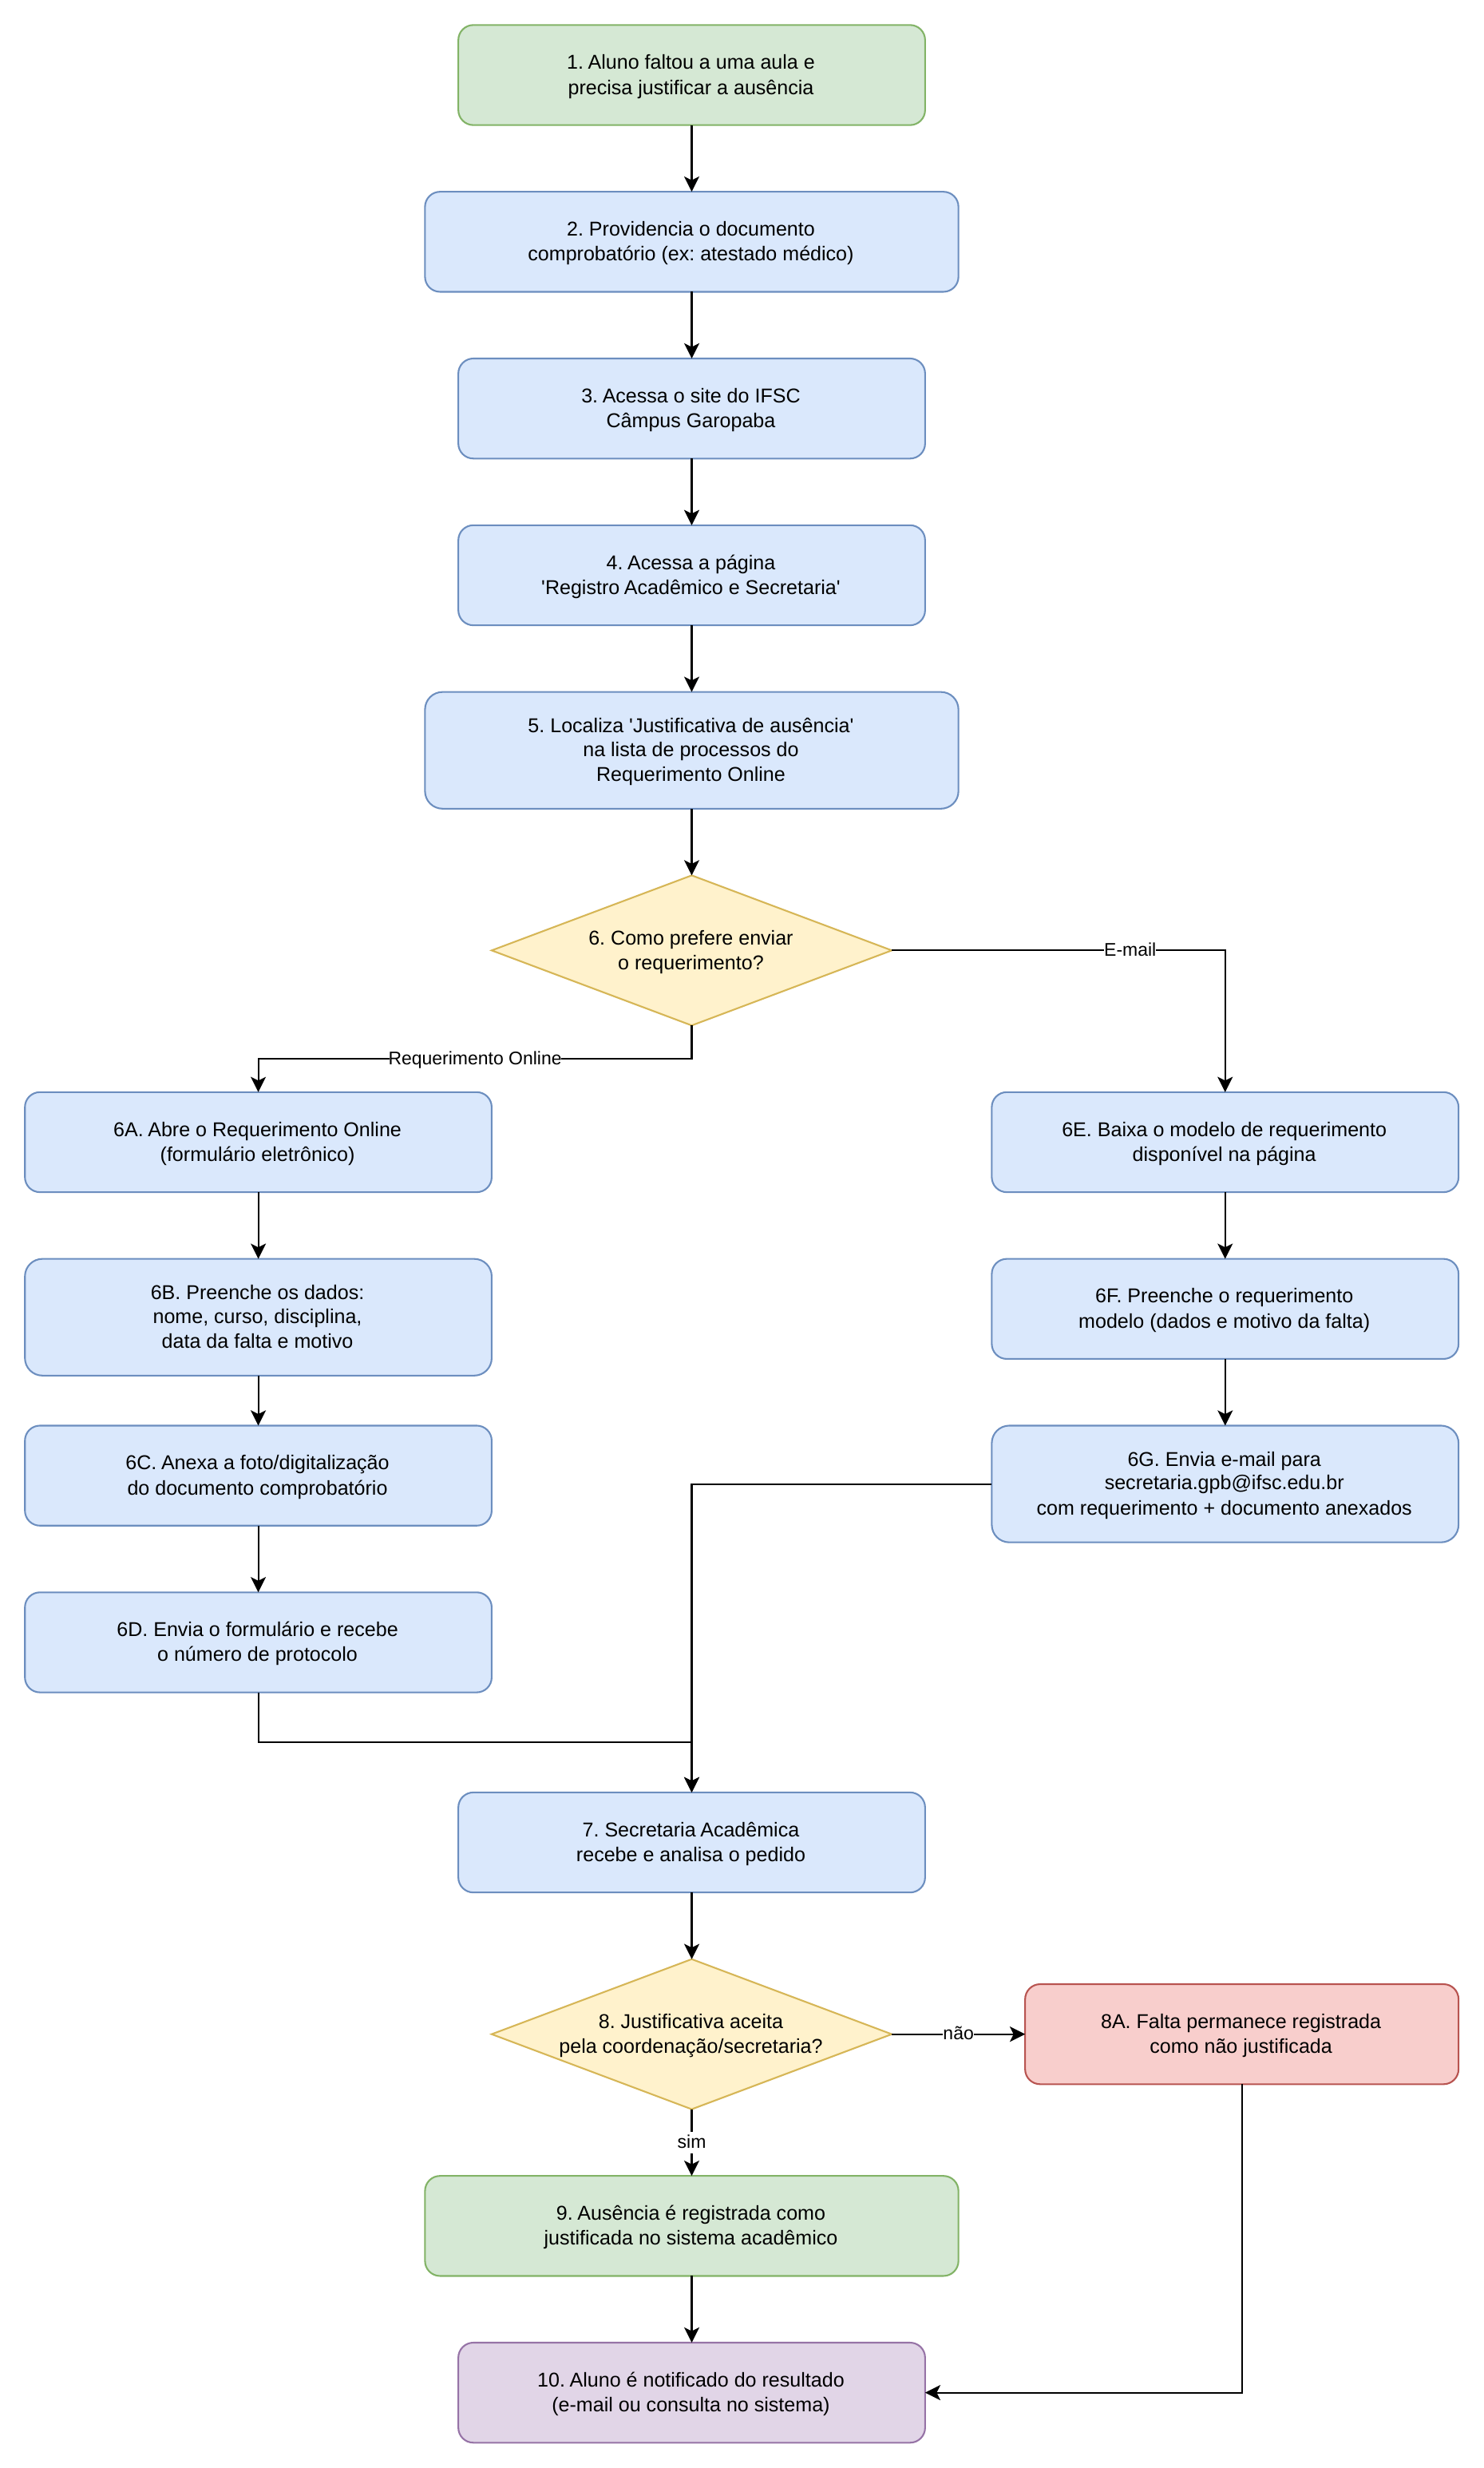
\includegraphics[width=\textwidth,height=0.80\textheight,keepaspectratio]{fluxo_justificativa_ausencia.png}
  \caption{Processo atual de justificativa de ausência no site do IFSC}
  \label{fig:justificativa}
\end{figure}
\begin{multicols}{2}


O segundo diagrama (Figura~\ref{fig:inscricao}) detalha o processo de \textbf{inscrição em um curso}
pelo Sistema de Ingresso do IFSC: leitura do edital, acesso ao sistema,
seleção do câmpus e do curso, cadastro ou atualização de dados pessoais,
preenchimento de questionário socioeconômico e de cotas, confirmação da
inscrição e conferência do comprovante -- um processo com mais de quinze
etapas até a confirmação efetiva da inscrição.

\end{multicols}
\begin{figure}[H]
  \centering
  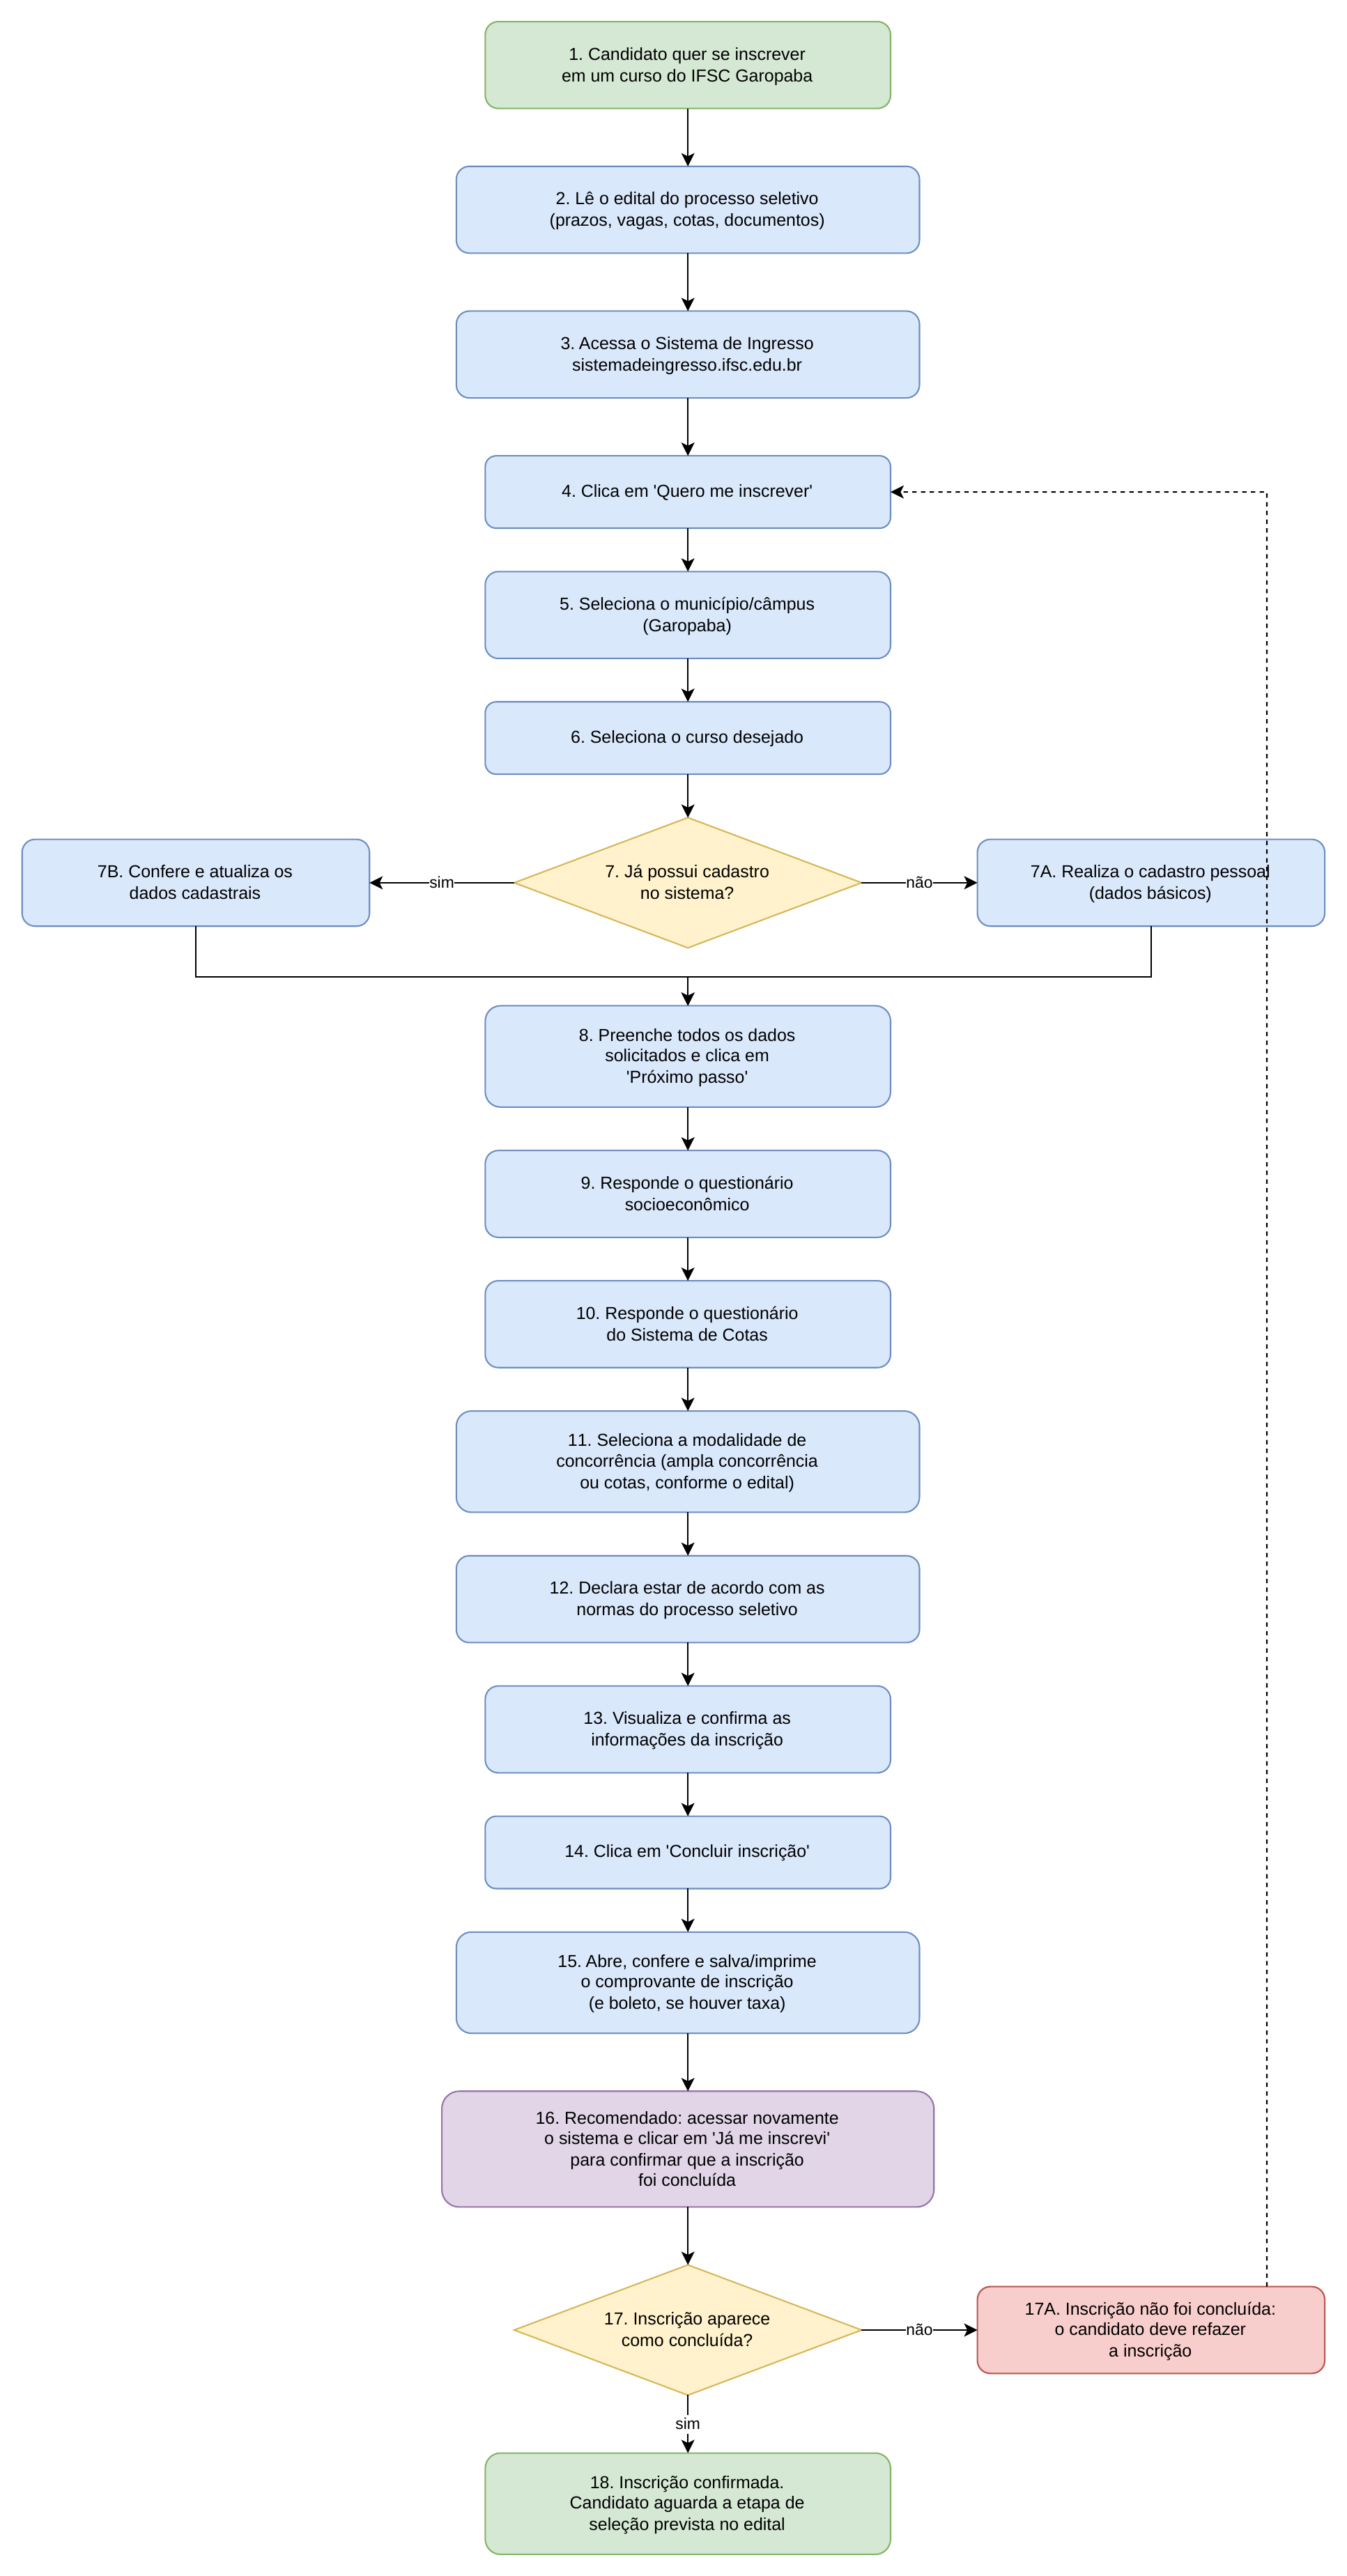
\includegraphics[width=\textwidth,height=0.80\textheight,keepaspectratio]{fluxo_inscricao_curso.png}
  \caption{Processo atual de inscrição em curso pelo Sistema de Ingresso}
  \label{fig:inscricao}
\end{figure}
\begin{multicols}{2}


O terceiro diagrama (Figura~\ref{fig:matricula}) amplia esse fluxo até a \textbf{efetivação da
matrícula}, cobrindo desde a consulta aos cursos ofertados e a
verificação de editais abertos até a etapa de seleção (sorteio, prova ou
sistemas unificados, conforme o edital), a divulgação do resultado, a
convocação para matrícula, o envio e a análise da documentação exigida, e a confirmação final da matrícula.



Esse mapeamento evidencia que, mesmo quando a informação já está
disponível nos sistemas oficiais do IFSC, o caminho até ela é longo e
pouco intuitivo para quem não está familiarizado com a estrutura do
site institucional -- reforçando a relevância de um chatbot capaz de
sintetizar essas etapas em respostas diretas e objetivas.

\end{multicols}
\begin{figure}[H]
  \centering
  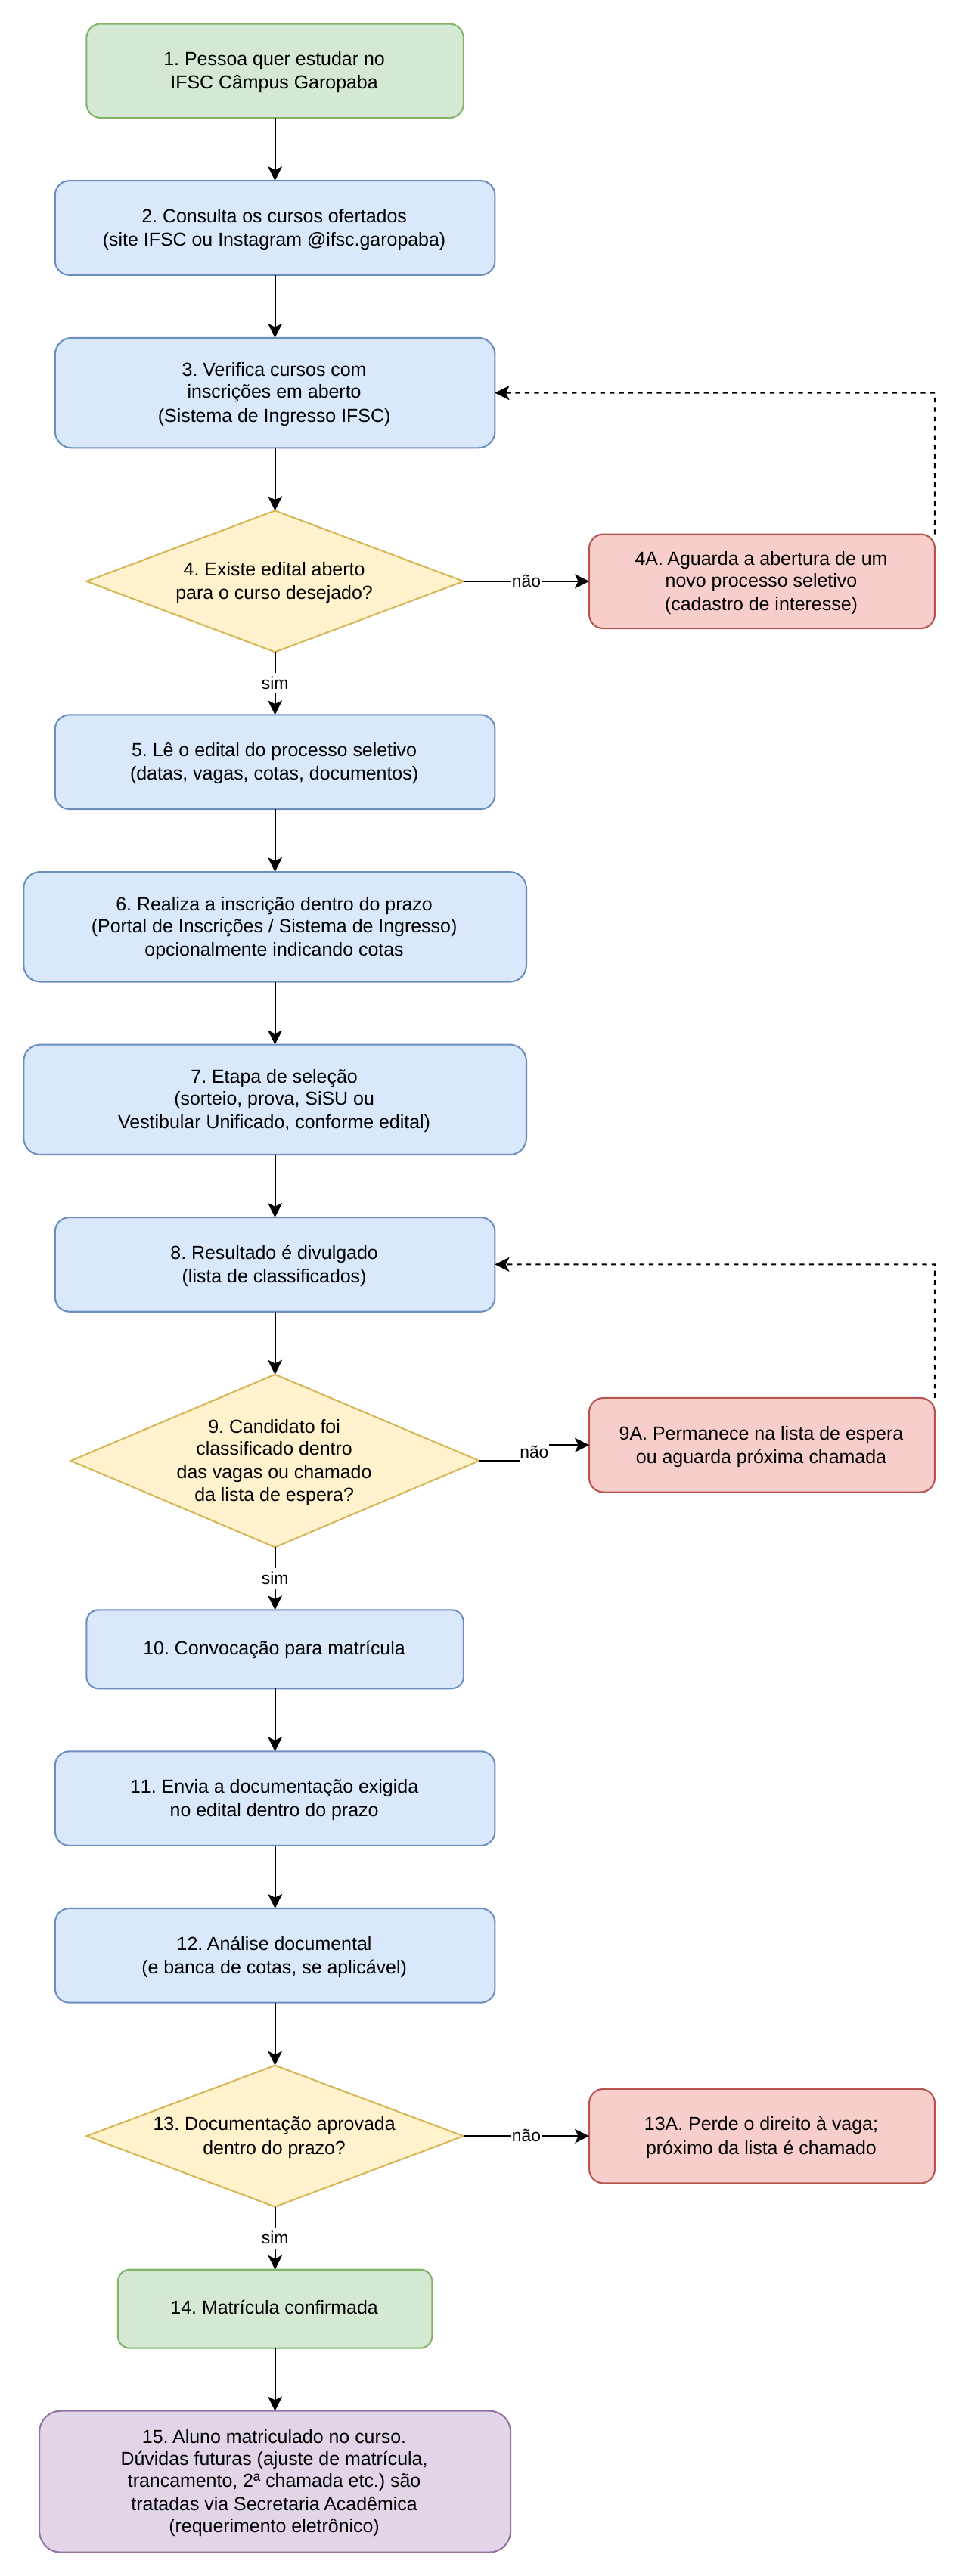
\includegraphics[width=\textwidth,height=0.80\textheight,keepaspectratio]{fluxo_curso_matricula.png}
  \caption{Processo atual do curso até a efetivação da matrícula}
  \label{fig:matricula}
\end{figure}
\begin{multicols}{2}


\section{Desenvolvimento do Chatbot}\label{sec:desenvolvimento}

O chatbot foi desenvolvido em Python, utilizando o framework Flask para o
gerenciamento das rotas e da interface web de conversação. A lógica de
atendimento foi definida a partir de um diagrama de fluxo (Figura~\ref{fig:fluxo_chatbot}),
elaborado ainda na fase de modelagem, que orienta toda a navegação do
usuário dentro do sistema. Nas subseções seguintes, são descritos a arquitetura e as tecnologias empregadas, a interface e a comunicação com o servidor, a persistência dos dados e o controle de acesso e, em seguida, o próprio fluxo de atendimento: o fluxo guiado por menus, o tratamento de texto livre, o encerramento do atendimento e o painel de controle de demandas.

\end{multicols}
\begin{figure}[H]
  \centering
  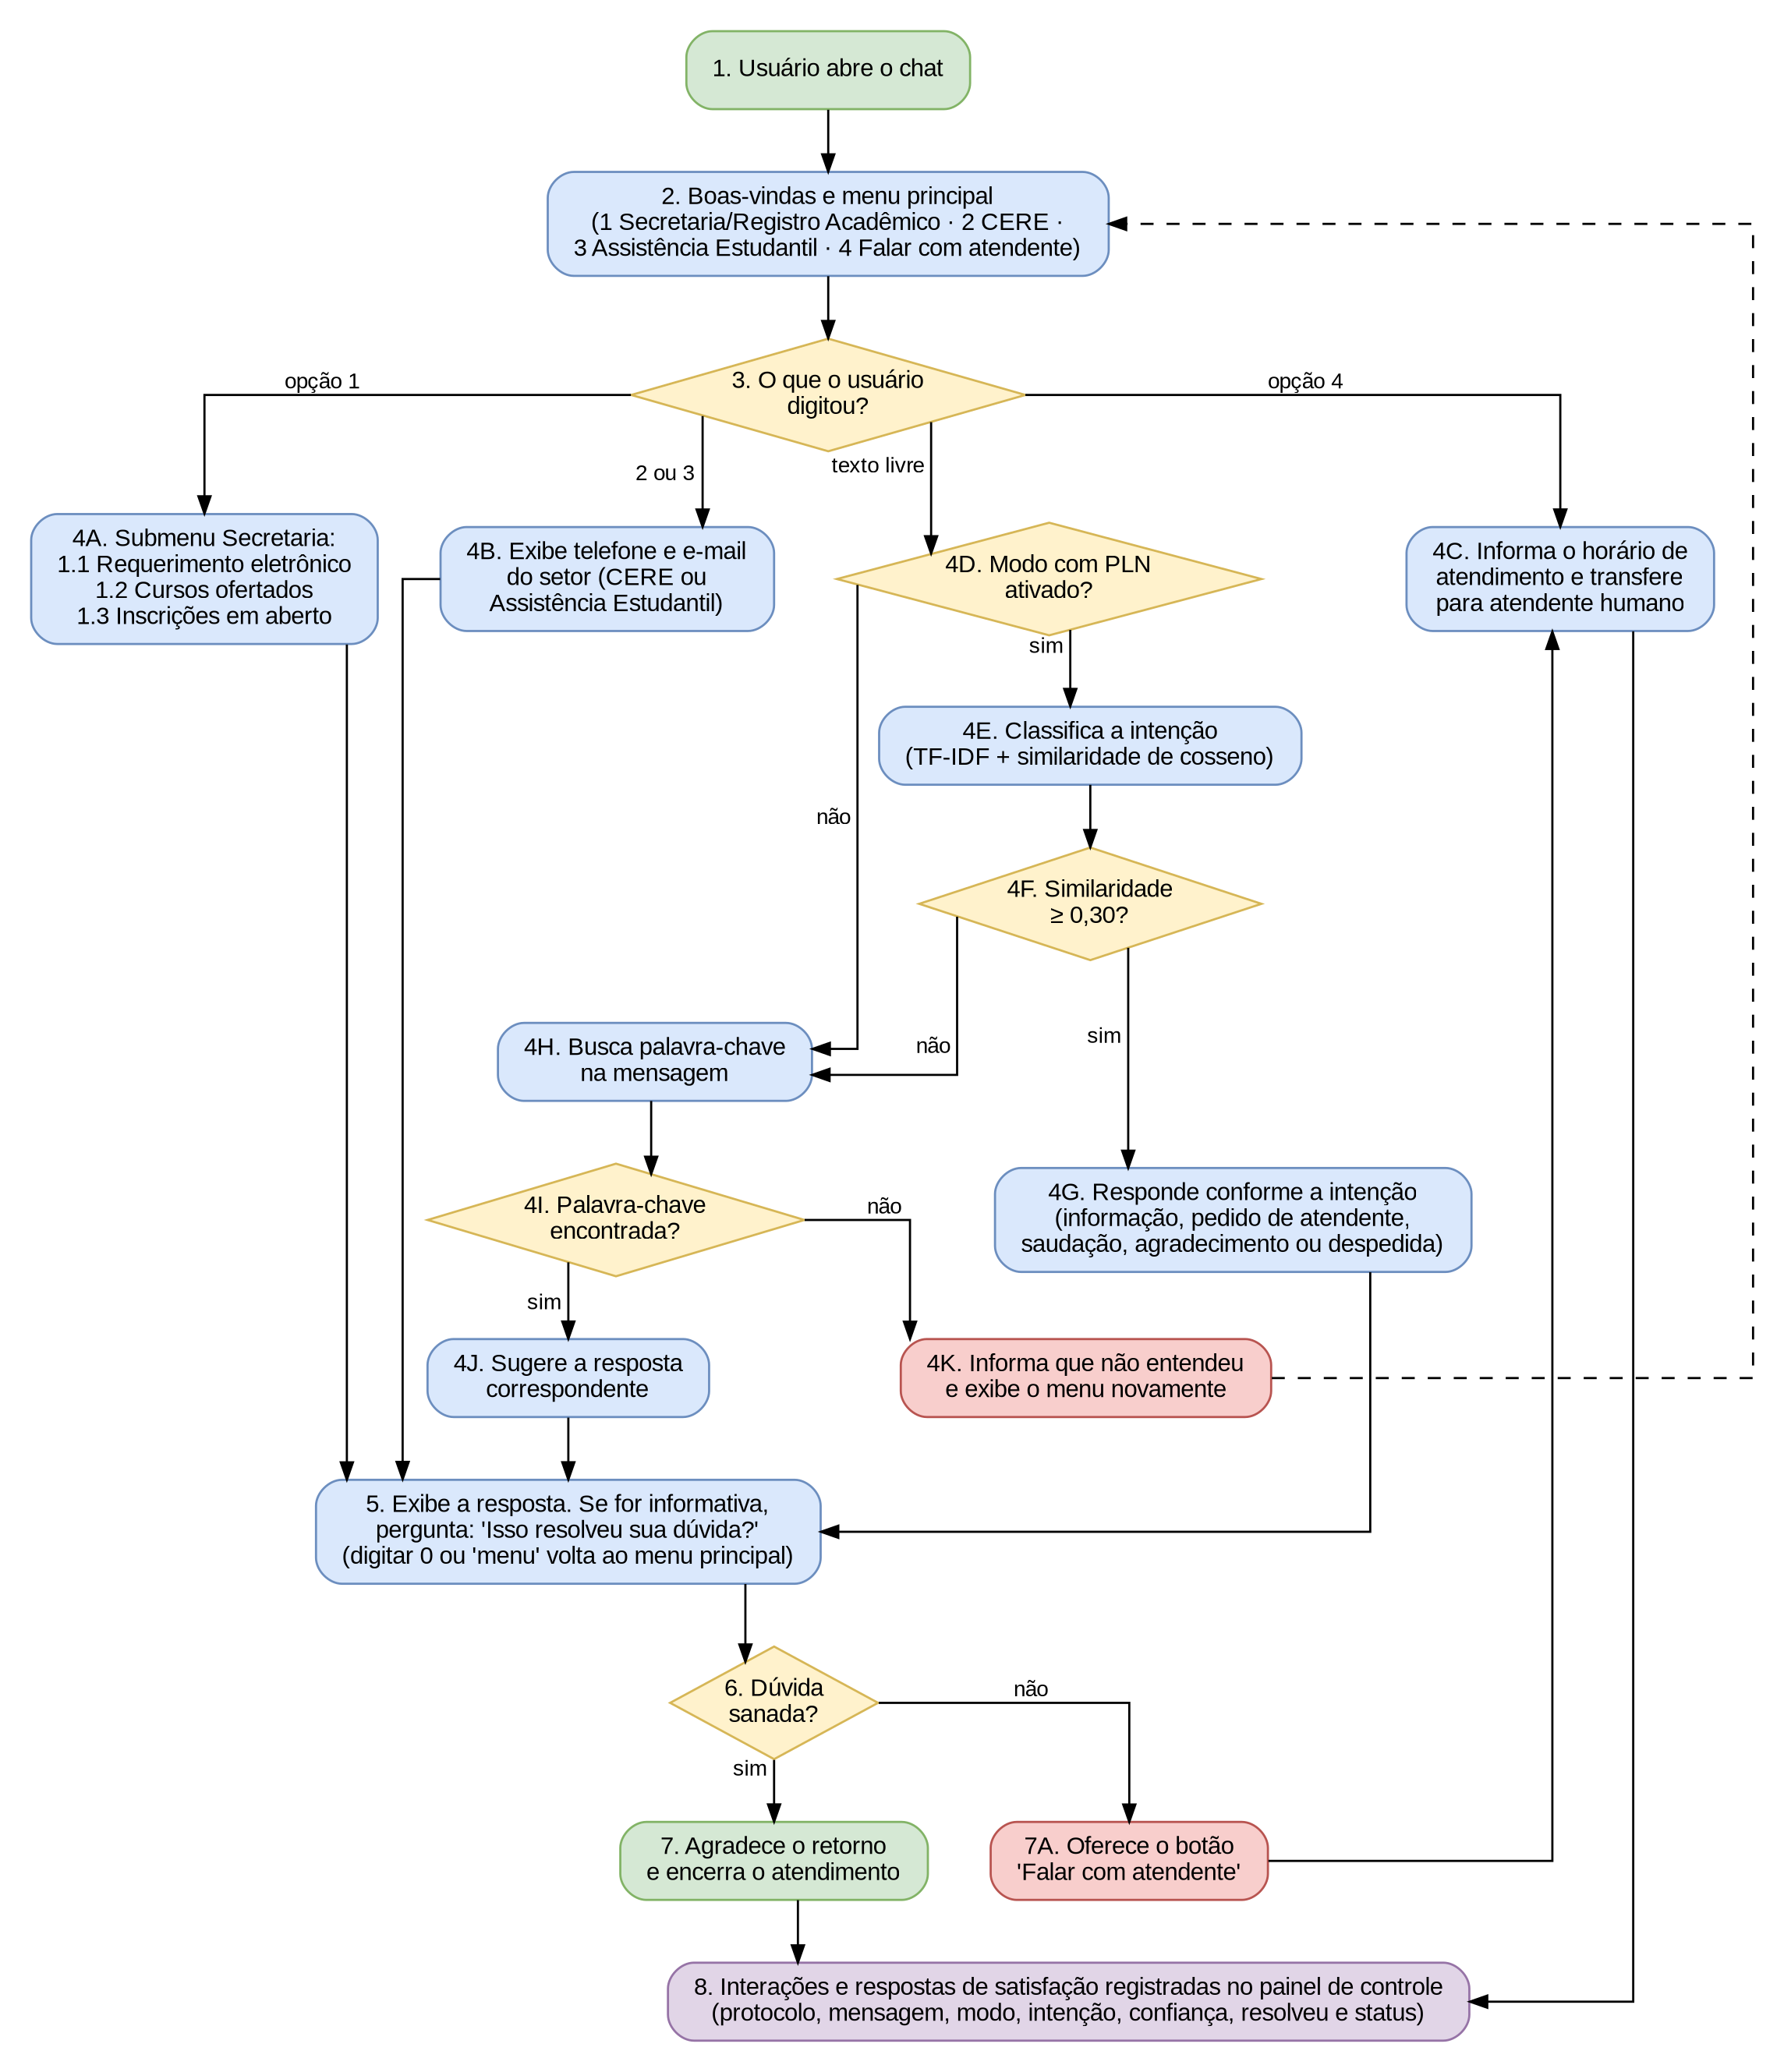
\includegraphics[width=\textwidth,height=0.80\textheight,keepaspectratio]{fluxo_chatbot.png}
  \caption{Fluxo de decisão do chatbot da Secretaria Acadêmica}
  \label{fig:fluxo_chatbot}
\end{figure}
\begin{multicols}{2}

\subsection{Arquitetura e Tecnologias Utilizadas}\label{sec:arquitetura}

O protótipo foi organizado em camadas com responsabilidades bem separadas,
conforme ilustrado na Figura~\ref{fig:arquitetura}. Na camada de apresentação,
o aluno e o atendente interagem por meio do navegador, em páginas escritas em
HTML, CSS e JavaScript. Essas páginas se comunicam com o servidor,
desenvolvido com o framework Flask, que recebe as requisições, aciona o núcleo
do chatbot e registra cada interação no banco de dados. O núcleo do chatbot
concentra a lógica de atendimento (estado da conversa, menus e ordem de
prioridade na interpretação das mensagens) e consulta dois componentes: o
módulo de conteúdo, que reúne os textos das respostas, os menus e as
palavras-chave, e o módulo de PLN, responsável por classificar a intenção das
mensagens em texto livre. Essa separação faz com que o núcleo do chatbot não
dependa do canal de atendimento: ele recebe apenas um identificador de usuário
e o texto da mensagem e devolve a resposta, o que permitiria reaproveitá-lo,
em trabalhos futuros, em outros canais, como o WhatsApp, bastando criar uma
nova rota no servidor.

\end{multicols}
\begin{figure}[H]
  \centering
  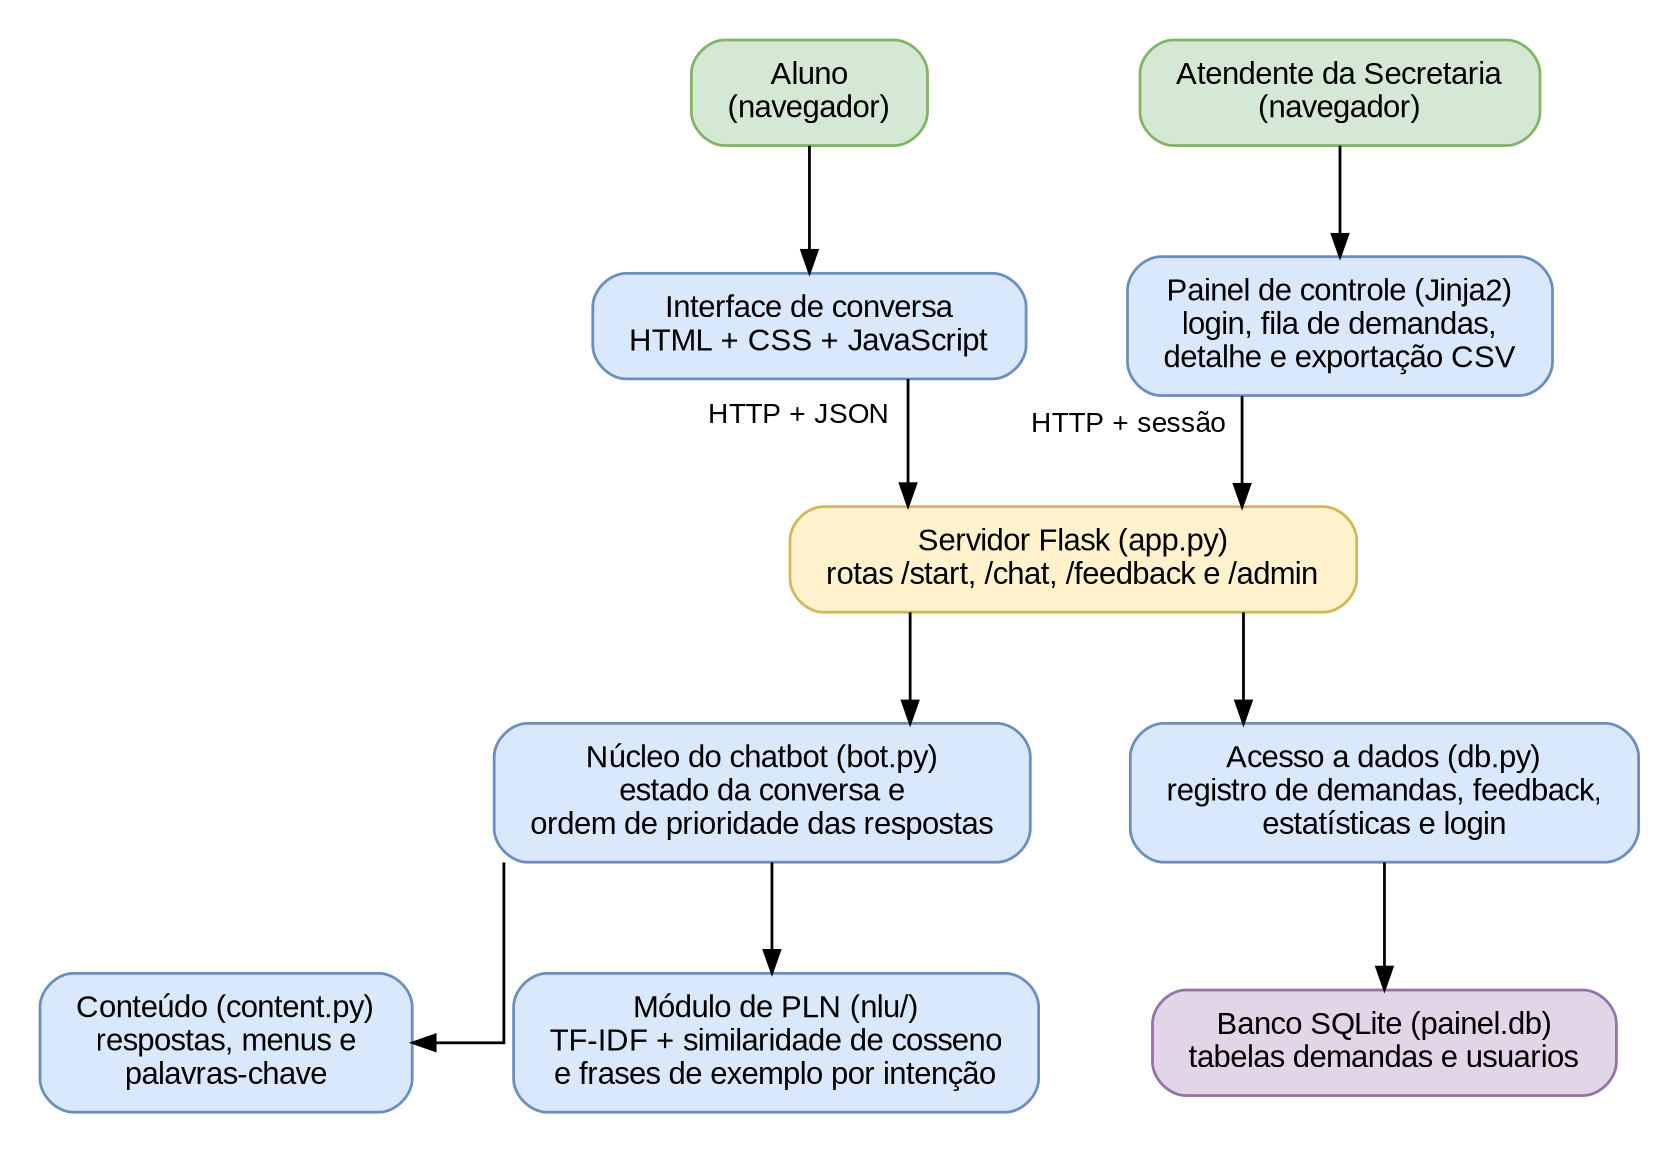
\includegraphics[width=0.92\textwidth]{arquitetura_sistema.png}
  \caption{Arquitetura do protótipo do chatbot e do painel de controle}
  \label{fig:arquitetura}
\end{figure}
\begin{multicols}{2}

O desenvolvimento utilizou a linguagem Python e priorizou, desde o início, o
uso de poucas dependências externas. A única biblioteca que precisa ser
instalada é o Flask (versão 3 ou superior), que fornece o servidor web, o
roteamento das requisições, o gerenciamento de sessão e o mecanismo de
\textit{templates} Jinja2, usado para gerar as páginas do painel. A biblioteca
Werkzeug, instalada junto com o Flask, é utilizada para o armazenamento seguro
de senhas. Todo o restante vem da biblioteca padrão do Python: o módulo
\texttt{sqlite3}, para o banco de dados; \texttt{csv} e \texttt{io}, para a
exportação dos dados; e \texttt{unicodedata}, \texttt{re}, \texttt{math} e
\texttt{collections}, para o tratamento de texto e o cálculo do classificador
de intenções. O \textit{front-end} foi escrito em HTML, CSS e JavaScript puros,
sem \textit{frameworks} nem bibliotecas externas, usando a função
\texttt{fetch} do navegador para trocar mensagens em formato JSON com o
servidor. Essa escolha mantém o sistema leve, simples de instalar e executável
em computadores com restrições de segurança, que costumam bloquear bibliotecas
com arquivos compilados -- razão pela qual o classificador de intenções foi
implementado em Python puro, em vez de utilizar bibliotecas de aprendizado de
máquina como o \textit{scikit-learn}. A Tabela~\ref{tab:modulos} resume a
responsabilidade de cada arquivo do projeto.

\end{multicols}
\begin{table}[H]
  \centering
  \begin{tabular}{|p{0.36\textwidth}|p{0.54\textwidth}|}
    \hline
    \textbf{Arquivo} & \textbf{Responsabilidade} \\ \hline
    \texttt{app.py} & Servidor Flask: rotas do chat, do feedback e do painel,
    exportação de dados e autenticação \\ \hline
    \texttt{bot.py} & Núcleo do chatbot: estado da conversa, menus e ordem de
    prioridade na interpretação das mensagens \\ \hline
    \texttt{content.py} & Textos das respostas, menus e lista de palavras-chave \\ \hline
    \texttt{nlu/classifier.py} & Classificador de intenções (TF-IDF e
    similaridade de cosseno) \\ \hline
    \texttt{nlu/training\_data.py} & Frases de exemplo de cada intenção \\ \hline
    \texttt{db.py} & Acesso ao banco SQLite: demandas, feedback, estatísticas e
    login \\ \hline
    \texttt{templates/} & Páginas HTML: conversa, login, painel e detalhe da
    demanda \\ \hline
  \end{tabular}
  \caption{Principais arquivos do protótipo e suas responsabilidades}
  \label{tab:modulos}
\end{table}
\begin{multicols}{2}

\subsection{Interface Web e Comunicação com o Servidor}\label{sec:api}

A interface de conversa é uma única página web, com uma janela de mensagens, um
campo de texto e um seletor que permite ligar ou desligar o modo com PLN
durante a conversa -- recurso criado para comparar os dois comportamentos nos
testes. Ao carregar a página, o navegador gera um identificador aleatório para
aquela sessão de conversa. O sistema não solicita \textit{login}, nome ou
matrícula ao aluno, de modo que nenhum dado pessoal é coletado além do que o
próprio usuário escreve nas mensagens.

A comunicação com o servidor ocorre por requisições HTTP com dados em formato
JSON, por meio das rotas resumidas na Tabela~\ref{tab:rotas}. Ao abrir a
página, o navegador solicita as boas-vindas à rota \texttt{/start}; a cada
mensagem enviada, chama a rota \texttt{/chat}, que devolve a resposta do
chatbot juntamente com a intenção reconhecida, o grau de confiança, o modo de
operação, o número de protocolo da demanda e a indicação de se a pergunta de
satisfação deve ser exibida; e, quando o usuário responde a essa pergunta, o
resultado é enviado à rota \texttt{/feedback}. O servidor valida as
requisições, rejeitando mensagens vazias ou sem identificador de usuário. O
botão ``Falar com atendente'', exibido quando o usuário informa que a dúvida não
foi sanada, envia ao servidor um comando interno, reconhecido em qualquer ponto
da conversa -- diferentemente da opção 4 do menu, que só é reconhecida no menu
principal.

\end{multicols}
\begin{table}[H]
  \centering
  \begin{tabular}{|p{0.30\textwidth}|p{0.11\textwidth}|p{0.43\textwidth}|}
    \hline
    \textbf{Rota} & \textbf{Método} & \textbf{Função} \\ \hline
    \texttt{/} & GET & Página de conversa com o chatbot \\ \hline
    \texttt{/start} & POST & Inicia a conversa e devolve as boas-vindas e o menu
    principal \\ \hline
    \texttt{/chat} & POST & Recebe a mensagem, devolve a resposta e registra a
    demanda \\ \hline
    \texttt{/feedback} & POST & Registra se a dúvida foi resolvida \\ \hline
    \texttt{/admin/login} e \texttt{/admin/logout} & GET e POST & Entrada e
    saída do atendente \\ \hline
    \texttt{/admin}$^{*}$ & GET & Painel: indicadores, filtros e fila de demandas \\ \hline
    \texttt{/admin/demanda/<id>}$^{*}$ & GET e POST & Detalhe da demanda;
    alteração de status e parecer \\ \hline
    \texttt{/admin/export}$^{*}$ & GET & Exportação das demandas em CSV \\ \hline
  \end{tabular}
  \caption{Rotas do servidor Flask ($^{*}$ exigem autenticação)}
  \label{tab:rotas}
\end{table}
\begin{multicols}{2}

O núcleo do chatbot mantém, em memória, o ponto do menu em que cada usuário se
encontra (menu principal ou submenu da Secretaria), o que permite interpretar
corretamente os números digitados em cada contexto. Como esse estado fica
apenas em memória, ele é reiniciado quando o servidor é reiniciado -- uma
limitação aceitável para o protótipo, mas que precisaria ser tratada em um
sistema em produção.

\subsection{Persistência de Dados e Controle de Acesso}\label{sec:dados}

Todas as interações são gravadas em um banco de dados SQLite, armazenado em um
único arquivo local e acessado pelo módulo \texttt{sqlite3} da biblioteca
padrão do Python, sem uso de mapeamento objeto-relacional. O SQLite dispensa a
instalação de um servidor de banco de dados, o que simplifica a implantação do
protótipo; e, como o acesso aos dados foi isolado em um único módulo, uma
eventual migração para um sistema gerenciador mais robusto, como PostgreSQL ou
MySQL, exigiria poucas mudanças no restante da aplicação. O banco possui duas
tabelas: \texttt{demandas}, em que cada mensagem trocada com o chatbot gera um
registro (Tabela~\ref{tab:demandas}), e \texttt{usuarios}, que guarda as
credenciais dos atendentes autorizados a acessar o painel. Os valores
informados pelos usuários são sempre repassados ao banco como parâmetros das
consultas, e não concatenados ao texto SQL, o que protege o sistema contra
injeção de SQL. Quando novos campos foram incorporados ao longo do
desenvolvimento (como a intenção detectada, o modo de operação e a resposta de
satisfação), foi implementada uma migração leve, que adiciona as colunas
ausentes ao iniciar o sistema e preserva os registros já existentes.

\end{multicols}
\begin{table}[H]
  \centering
  \begin{tabular}{|p{0.34\textwidth}|p{0.56\textwidth}|}
    \hline
    \textbf{Campo} & \textbf{Descrição} \\ \hline
    \texttt{id} & Número de protocolo da demanda \\ \hline
    \texttt{user\_id} & Identificador aleatório da sessão de conversa \\ \hline
    \texttt{mensagem}, \texttt{resposta\_bot} & Texto enviado pelo usuário e
    resposta apresentada pelo chatbot \\ \hline
    \texttt{data\_hora} & Data e hora do registro \\ \hline
    \texttt{modo} & Modo de operação (com PLN ou somente palavras-chave) \\ \hline
    \texttt{intent\_detectado}, \texttt{confianca} & Intenção reconhecida e
    grau de similaridade (de 0 a 1), quando há \\ \hline
    \texttt{resolvido\_pelo\_usuario} & Resposta à pergunta de satisfação (Sim
    ou Não) \\ \hline
    \texttt{status} & Pendente, Em análise ou Resolvido \\ \hline
    \texttt{parecer}, \texttt{atendente} & Observação registrada e responsável
    pela atualização \\ \hline
  \end{tabular}
  \caption{Campos da tabela \texttt{demandas}}
  \label{tab:demandas}
\end{table}
\begin{multicols}{2}

O acesso ao painel da Secretaria é restrito a atendentes autenticados. As
páginas administrativas são protegidas por uma verificação de sessão: quem
tenta acessá-las sem estar autenticado é redirecionado à tela de \textit{login}.
As senhas não são armazenadas em texto puro, mas sob a forma de \textit{hash},
gerado pela biblioteca Werkzeug, e a sessão do atendente é assinada com uma
chave secreta do Flask e encerrada ao sair. Essa proteção é relevante porque o
painel reúne mensagens dos alunos, que podem conter informações pessoais, e
dialoga com os cuidados exigidos pela Lei Geral de Proteção de Dados (LGPD).
Por se tratar de um protótipo, o usuário inicial, criado automaticamente na
primeira execução, e a chave de sessão são valores padrão, que devem ser
substituídos antes de uma implantação real.

\subsection{Fluxo Guiado por Menus}

Ao iniciar a conversa, o usuário recebe uma mensagem de boas-vindas
seguida do menu principal, com quatro opções: (1) Secretaria/Registro
Acadêmico, (2) CERE, (3) Assistência Estudantil e (4) Falar com
atendente. A opção de Secretaria/Registro Acadêmico direciona a um
submenu específico, com respostas sobre requerimento eletrônico, cursos
ofertados e inscrições em aberto -- assuntos identificados como os mais
recorrentes na entrevista com a Secretaria (Seção~\ref{sec:entrevista}). As demais opções do
menu principal retornam informações de contato (telefone e e-mail) dos
respectivos setores ou encaminham o usuário para um atendente humano,
informando o horário de atendimento. Ao final de cada resposta, o
sistema exibe a instrução \textit{``Digite 0 para voltar ao menu
principal''}, permitindo que o usuário continue navegando sem reiniciar a
conversa. A Figura~\ref{fig:telas} apresenta as telas do chatbot nesse fluxo.

\end{multicols}
\begin{figure}[H]
  \centering
  \begin{minipage}[t]{0.46\textwidth}
    \centering
    {\setlength{\fboxsep}{0pt}\fbox{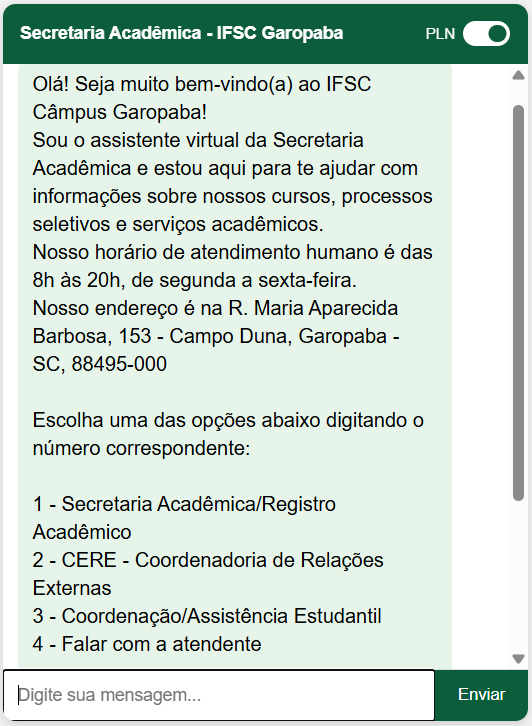
\includegraphics[width=0.97\linewidth]{tela_principal.png}}}\\[3pt]
    {\small (a)}
  \end{minipage}\hfill
  \begin{minipage}[t]{0.46\textwidth}
    \centering
    {\setlength{\fboxsep}{0pt}\fbox{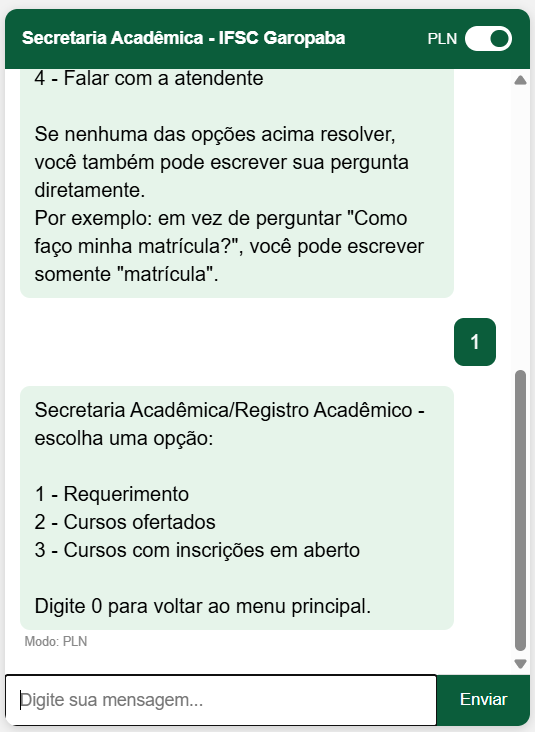
\includegraphics[width=0.97\linewidth]{tela_opcao_1.png}}}\\[3pt]
    {\small (b)}
  \end{minipage}

  \vspace{1.2em}

  \begin{minipage}[t]{0.46\textwidth}
    \centering
    {\setlength{\fboxsep}{0pt}\fbox{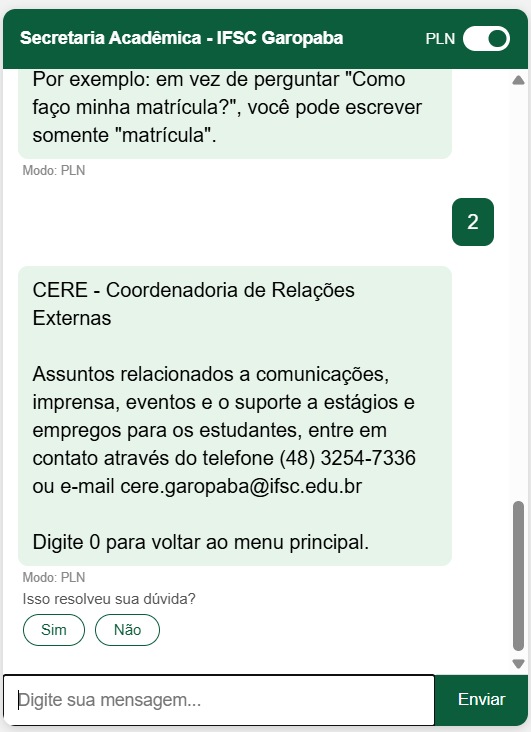
\includegraphics[width=0.97\linewidth]{tela_opcao_2.png}}}\\[3pt]
    {\small (c)}
  \end{minipage}\hfill
  \begin{minipage}[t]{0.46\textwidth}
    \centering
    {\setlength{\fboxsep}{0pt}\fbox{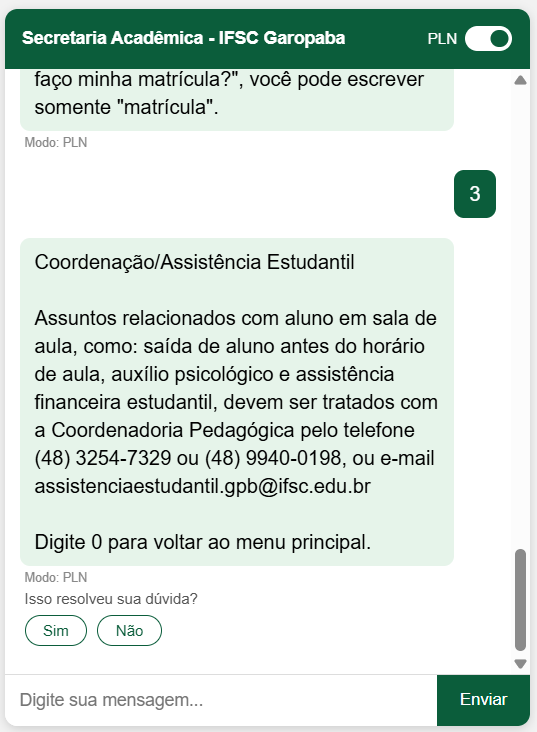
\includegraphics[width=0.97\linewidth]{tela_opcao_3.png}}}\\[3pt]
    {\small (d)}
  \end{minipage}
  \caption{Telas do chatbot no fluxo guiado por menus: (a) mensagem de boas-vindas e menu principal; (b) submenu da Secretaria Acadêmica/Registro Acadêmico; (c) resposta da opção CERE, com a pergunta de satisfação; (d) resposta da opção Coordenação/Assistência Estudantil}
  \label{fig:telas}
\end{figure}
\begin{multicols}{2}


\subsection{Tratamento de Texto Livre}\label{sec:textolivre}

Quando o usuário digita uma mensagem fora das opções numéricas do menu, o
sistema recorre ao módulo de interpretação de texto livre. Esse módulo foi
implementado com duas opções de operação, selecionáveis por meio de um
botão na interface: o modo \textit{apenas com palavras-chave} e o modo
\textit{com PLN}. Essa divisão permite comparar, durante os testes do
protótipo, o comportamento do sistema com e sem o tratamento de linguagem
natural. Em qualquer dos modos, os números do menu e o comando ``menu'' têm
prioridade e são tratados diretamente, sem interpretação de texto.

No modo com palavras-chave, a mensagem é normalizada (conversão para
minúsculas e remoção de acentos) e o sistema procura nela, por
correspondência de trecho, uma das 43 palavras-chave cadastradas,
associadas às demandas mais comuns levantadas na entrevista (como
``matrícula'', ``diploma'', ``curso'', entre outras). Se uma palavra-chave é
identificada, o chatbot sugere a resposta correspondente; caso nenhuma
seja encontrada, informa que não compreendeu a mensagem e exibe o menu
novamente, para que o usuário prossiga pela navegação guiada. Quando a
palavra-chave indica um pedido de atendente humano (como ``atendente'' ou
``humano''), o bot reforça o menu principal e orienta o usuário a digitar a
opção 4.

No modo com PLN, a mensagem é primeiro submetida a um classificador de
intenções, implementado em Python sem bibliotecas externas de aprendizado
de máquina, a partir das técnicas de TF-IDF e similaridade de cosseno
(Seção~\ref{sec:pln}). A base do classificador é um conjunto de 141 frases
de exemplo, distribuídas em 13 intenções: as seis respostas informativas
do chatbot, o pedido de atendente, quatro tipos de saudação, o
agradecimento e a despedida. Cada frase é convertida em um vetor que
considera palavras isoladas e pares de palavras vizinhas, com maior peso
para os termos mais raros; a mensagem do usuário recebe a mesma
representação e é comparada com todas as frases de exemplo, adotando-se a
intenção da mais semelhante, desde que a similaridade alcance o limiar de
0,30. Abaixo desse valor, o sistema prefere não arriscar uma resposta e
recorre à busca por palavras-chave descrita acima, que atua como rede de
segurança.

Não há uma etapa de treinamento separada: o índice é montado em memória
quando o servidor inicia, de modo que ampliar o conjunto de exemplos exige
apenas editar o arquivo de frases. A opção por uma implementação em Python
puro mantém o sistema leve e evita problemas de execução em computadores
cujas políticas de segurança bloqueiam bibliotecas compiladas.

A resposta do chatbot pode ter dois níveis de detalhe. Para a maioria dos
serviços de requerimento, a resposta é uma lista geral dos assuntos
tratados pela Secretaria, com o link do requerimento eletrônico (opção 1.1
do menu). Já a justificativa de ausência, uma das dúvidas mais frequentes
relatadas na entrevista, possui uma intenção própria: quando o usuário
pergunta sobre faltas, o chatbot responde diretamente com o procedimento
resumido -- solicitar a justificativa pelo Requerimento Online anexando o
documento comprobatório, ou enviar o modelo de requerimento por e-mail à
secretaria --, em vez de apresentar a lista completa. Essa separação foi
motivada por um teste do protótipo em que a mensagem ``faltei ontem'' era
corretamente associada ao grupo de requerimentos, mas recebia como
resposta uma lista extensa, sem o passo a passo do serviço desejado.

Na prática, a diferença entre os modos aparece em mensagens que não contêm
uma palavra-chave exata. A mensagem ``faltei ontem e quero justificar'', por
exemplo, é associada pelo classificador à intenção de justificativa de
ausência, e ``não pude ir à aula por doença'', que não contém nenhuma das
palavras-chave cadastradas, também é reconhecida no modo com PLN; já as saudações e agradecimentos (como ``bom dia'' e ``obrigada''), só são
reconhecidos no modo com PLN.

Para orientar usuários com pouca familiaridade com chatbots, a mensagem do
menu informa que, se nenhuma opção resolver a dúvida, é possível escrever
a pergunta diretamente, acompanhada de um exemplo de uso: em vez de ``Como
faço minha matrícula?'', basta digitar ``matrícula''.

\subsection{Encerramento do Atendimento}

Após uma resposta informativa -- isto é, uma informação efetivamente
fornecida, e não apenas a abertura de um menu, uma saudação ou um pedido
de atendente --, o chatbot pergunta ao usuário se a dúvida ou o
questionamento apresentado foi sanado, oferecendo duas opções de resposta:
sim ou não. A pergunta é feita somente nesses casos para que a taxa de
resolução não seja distorcida por interações em que ela não faria sentido,
como cumprimentos e agradecimentos. Caso o usuário responda que sim, o
sistema agradece o retorno e o atendimento é encerrado. Caso responda que
não, o sistema registra a resposta, lamenta não ter ajudado e exibe o
botão ``Falar com atendente'', que transfere o usuário para o atendimento
humano e informa o horário de funcionamento (das 8h às 20h, de segunda a
sexta-feira) -- de forma equivalente ao que hoje ocorre por WhatsApp,
porém de maneira registrada. A Figura~\ref{fig:atendente} mostra a mensagem exibida ao usuário nessa transferência, e a pergunta de satisfação, com os botões \textit{Sim} e \textit{Não}, pode ser vista nas Figuras~\ref{fig:telas}(c) e~\ref{fig:telas}(d). Todas essas interações são registradas no painel de controle, descrito na Seção~\ref{sec:painel}.

\begin{figure}[H]
  \centering
  {\setlength{\fboxsep}{0pt}\fbox{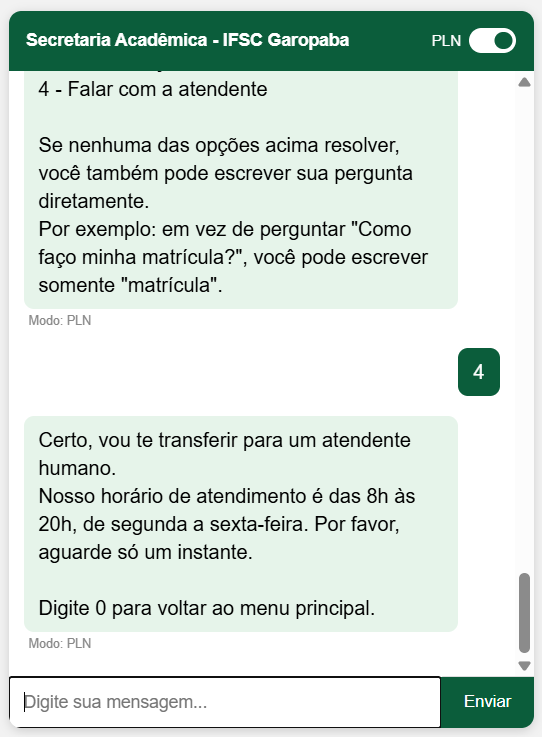
\includegraphics[width=0.85\columnwidth]{tela_opcao_4.png}}}
  \caption{Resposta do chatbot ao pedido de atendimento humano (opção 4 do menu principal)}
  \label{fig:atendente}
\end{figure}


\subsection{Painel de Controle de Demandas}\label{sec:painel}

O painel de controle foi criado para suprir a lacuna de métricas identificada
na entrevista com a Secretaria (Seção~\ref{sec:entrevista}): até então, não
havia como saber quantos atendimentos eram realizados, quantos eram concluídos
e sobre quais assuntos. Ele foi desenvolvido dentro da própria aplicação Flask
do chatbot, e não como um sistema à parte, de modo que os dois compartilham o
mesmo servidor e o mesmo banco de dados SQLite. A construção seguiu quatro
passos. Primeiro, definiu-se o que registrar: cada mensagem enviada ao chatbot
gera uma \textit{demanda}, com número de protocolo, data e hora, texto da
mensagem, resposta apresentada, modo de operação, intenção reconhecida e
resposta do usuário à pergunta de satisfação (Tabela~\ref{tab:demandas}).
Segundo, foram criadas, no módulo de acesso a dados, as funções para registrar,
listar, filtrar, atualizar e contar demandas e para calcular a taxa de
resolução por modo de operação. Terceiro, foram implementadas as rotas
administrativas e as páginas do painel, geradas por \textit{templates} Jinja2 e
mantidas na mesma identidade visual do chat (o verde institucional). Por fim,
o acesso foi protegido por autenticação, conforme descrito na
Seção~\ref{sec:dados}.

O painel é composto por três telas, resumidas na Tabela~\ref{tab:painel}.
Toda demanda nasce com o status \textit{Pendente}; o atendente a abre, analisa e
a classifica como \textit{Em análise} ou \textit{Resolvido}, registrando um
parecer que fica gravado junto com o nome do atendente responsável. Quando a
interação foi feita por navegação direta no menu, a coluna de intenção exibe
apenas ``menu'', pois nesses casos o classificador não é acionado.

\end{multicols}
\begin{table}[H]
  \centering
  \begin{tabular}{|p{0.20\textwidth}|p{0.70\textwidth}|}
    \hline
    \textbf{Tela} & \textbf{Componentes} \\ \hline
    Login & Formulário com usuário e senha; mensagem de erro quando as
    credenciais são inválidas. \\ \hline
    Fila de demandas (tela principal) &
    Cabeçalho com a saudação ao atendente e o botão de saída;
    quatro cartões de indicadores (total de demandas, pendentes, em análise e
    resolvidas); três cartões com a taxa de resolução informada pelos usuários
    (geral, modo com PLN e modo apenas com palavras-chave), com o percentual,
    o número de respostas \textit{sim} e \textit{não} e o total de avaliações,
    destacado em verde ou vermelho conforme esteja acima ou abaixo de 50\%;
    filtros por status e botão para exportar os dados em CSV; e tabela com
    protocolo, data e hora, identificador do usuário, mensagem, intenção
    reconhecida (com a confiança do classificador), indicação se a dúvida foi
    resolvida, status (em etiqueta colorida), atendente e link para abrir a
    demanda. \\ \hline
    Detalhe da demanda & Dados completos da interação (usuário, data e hora,
    mensagem, resposta do chatbot, intenção reconhecida e resposta de
    satisfação) e formulário de análise, com seleção de status, campo de texto
    para o parecer e botão de salvar, que registra o atendente logado como
    responsável e retorna à fila. \\ \hline
  \end{tabular}
  \caption{Telas do painel de controle e seus componentes}
  \label{tab:painel}
\end{table}
\begin{multicols}{2}

\IfFileExists{figures/painel_controle.png}{%
A Figura~\ref{fig:painel} apresenta a tela principal do painel.

\end{multicols}
\begin{figure}[H]
  \centering
  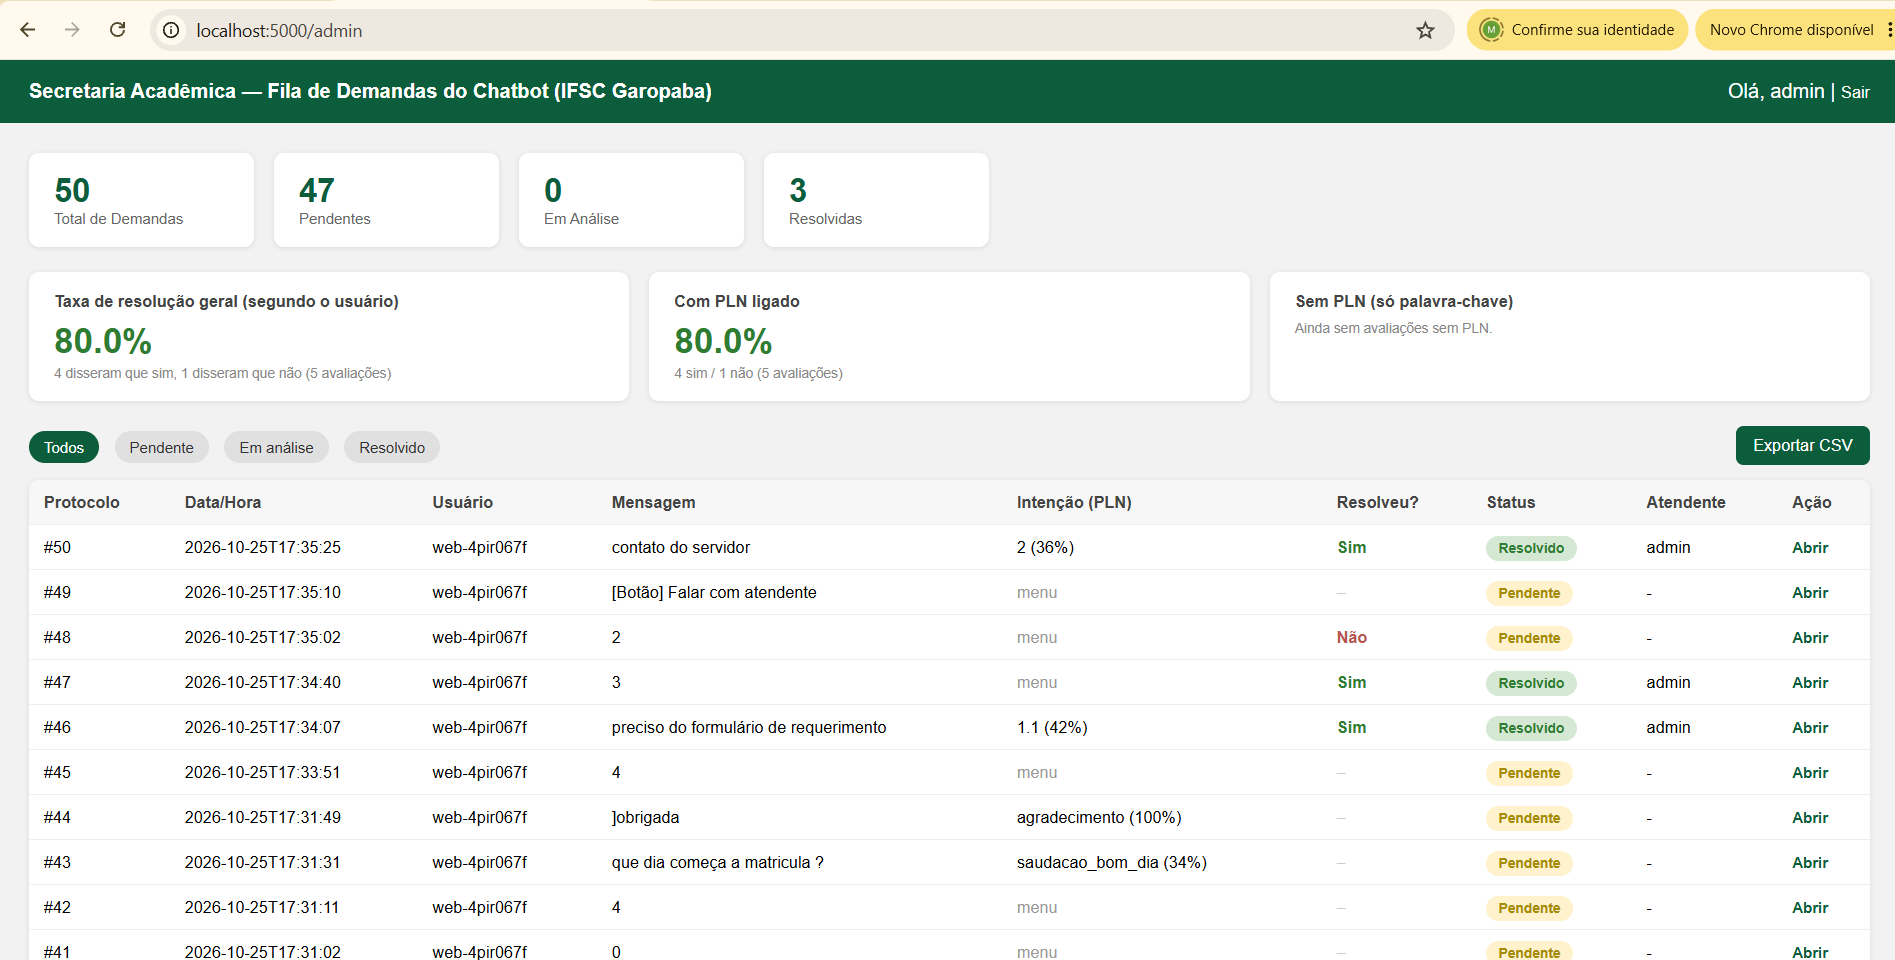
\includegraphics[width=\textwidth]{painel_controle.png}
  \caption{Painel de controle de demandas do chatbot}
  \label{fig:painel}
\end{figure}
\begin{multicols}{2}
}{}

A exportação em CSV reúne, para cada demanda, o protocolo, a data e hora, o
identificador do usuário, a mensagem, a resposta do chatbot, o modo de
operação, a intenção detectada e sua confiança, a resposta de satisfação, o
status, o parecer e o atendente, permitindo análises posteriores fora da
aplicação, como a comparação entre os modos com e sem PLN. Assim, o painel
permite à Secretaria Acadêmica visualizar, pela primeira vez, dados como o
volume de atendimentos realizados, a proporção de dúvidas resolvidas pelo
chatbot segundo os próprios usuários e os assuntos mais demandados pelos
estudantes.


\section{Resultados}\label{sec:resultados}

Até o presente momento, o protótipo encontra-se funcional em sua
totalidade em relação ao fluxo descrito na Seção~\ref{sec:desenvolvimento}: o menu guiado, o tratamento de texto livre (classificador de intenções com PLN e busca por palavras-chave), a alternância entre os modos com e sem PLN, o encerramento do atendimento com verificação de
satisfação e o registro das interações no painel de controle já estão
implementados e operantes.

Testes manuais indicam que o fluxo guiado por menus responde de forma
consistente e previsível a todas as opções mapeadas no diagrama de fluxo,
enquanto o módulo de interpretação de texto livre apresenta bom desempenho para mensagens que utilizam termos próximos aos cadastrados (como ``matrícula'' ou ``curso''). O modo com PLN reconhece ainda variações de escrita (como ``faltei ontem e quero justificar'') e mensagens de cortesia, como saudações e agradecimentos, que o modo apenas com palavras-chave não compreende. Em ambos os modos, porém, persistem limitações diante de mensagens com vocabulário muito diferente do previsto, nas quais o chatbot retorna o menu principal em vez de uma resposta específica.

O painel de controle já é capaz de registrar cada atendimento realizado
pelo chatbot, incluindo o protocolo, a mensagem recebida, a intenção reconhecida pelo módulo de PLN e se o usuário informou que a dúvida foi sanada ou não -- um retrato exatamente do tipo de dado que, segundo
relatado na entrevista (Seção~\ref{sec:entrevista}), inexiste no atendimento atual via
WhatsApp. Em uma rodada de testes realizada durante o desenvolvimento, o
painel registrou um total de 23 demandas, das quais 22 permaneceram
pendentes de triagem pelo atendente e 1 foi marcada como resolvida,
demonstrando que o fluxo de registro, classificação de status (pendente,
em análise, resolvido) e listagem das demandas funciona de ponta a ponta.
Uma avaliação mais formal, com um período de uso real por estudantes e
comparação entre os modos com e sem PLN, está prevista como etapa futura
do trabalho.

\subsection{Validação com o Servidor da Secretaria}

Em outubro de 2026, o protótipo foi apresentado ao servidor responsável
pela Secretaria Acadêmica, futuro usuário da ferramenta, com o objetivo
de verificar se a solução atendia às necessidades reais do setor. Durante
a apresentação, o servidor sugeriu um ajuste de usabilidade, já
incorporado ao sistema: na mensagem em que o chatbot informa que, caso
nenhuma das opções do menu resolva a dúvida, o usuário pode escrever a
pergunta diretamente, foi acrescentado um exemplo prático de como fazê-lo (Figura~\ref{fig:telas}(b))
-- em vez de digitar ``Como faço minha matrícula?'', o usuário pode
escrever apenas ``matrícula''. Segundo o servidor, a medida é importante
porque parte do público tem dificuldade em interagir com chatbots, seja
por falta de familiaridade com a ferramenta, seja por desconhecimento de
como formular a pergunta. Em seguida, o servidor avaliou o resultado de
forma positiva, destacando que o chatbot tem potencial para contribuir de
forma significativa com o seu trabalho, desafogando a rotina de
atendimento hoje concentrada no WhatsApp.

Embora se trate de uma validação qualitativa, realizada com um único
servidor e sem aplicação de instrumento formal de avaliação, esse retorno
é relevante por partir do próprio profissional que vivencia a demanda
descrita na Seção~\ref{sec:entrevista}, indicando que o protótipo está alinhado às
necessidades levantadas e que a abordagem adotada é aceita pelo público
a que se destina. Uma avaliação quantitativa, com base nos dados
registrados pelo painel de controle durante um período de uso real, segue
prevista como trabalho futuro.

\section{Considerações Finais}

Este trabalho apresentou o desenvolvimento de um chatbot voltado ao
atendimento da Secretaria Acadêmica do IFSC -- Campus Garopaba,
utilizando o framework leve Flask e um módulo de tratamento de texto livre baseado em classificação de intenções e busca por palavras-chave. A partir do levantamento de
requisitos junto ao setor, foi possível identificar não apenas as
principais demandas dos estudantes, mas também um problema estrutural do
atendimento atual: a completa ausência de métricas sobre o volume,
conclusão e natureza dos atendimentos realizados via WhatsApp -- lacuna
não abordada pelos trabalhos relacionados apresentados na Seção~\ref{sec:trabalhos}.

O protótipo desenvolvido contempla um fluxo guiado por menus, um módulo
de interpretação de texto livre com alternância entre os modos com e sem
PLN, oferta de encaminhamento a atendente humano quando a dúvida não é sanada, e um
painel de controle que registra cada interação. Os resultados
preliminares indicam que a proposta é viável e que uma solução leve,
baseada em menus, classificação de intenções por similaridade textual e busca por palavras-chave, já é suficiente para
atender parte significativa das demandas mapeadas, cumprindo os
objetivos específicos definidos na Seção~\ref{sec:objetivos}.

Como trabalhos futuros, pretende-se ampliar o conjunto de palavras-chave, de frases de exemplo e de respostas do módulo de PLN -- inclusive com respostas específicas por serviço, como a já implementada para a justificativa de ausência --, incorporar uma etapa de validação de
identidade do usuário (como a verificação de CPF observada no chatbot da
Ortoimagem de Tubarão, Seção~\ref{sec:metodologia}), realizar um período de testes com
estudantes e servidores reais do campus, e utilizar os dados coletados
pelo painel de controle para avaliar quantitativamente a efetividade do
chatbot frente ao atendimento tradicional por WhatsApp.

\section{Referências}

ANTICO, Chiara; GIORDANO, Stefano; KOYUTURK, Cansu; OGNIBENE, Dimitri.
Unimib Assistant: designing a student-friendly RAG-based chatbot for all
their needs. In: \textbf{Italian Workshop on Artificial Intelligence for
Human Machine Interaction (AIxHMI 2024)}, Bolzano, 2024. arXiv:2411.19554.
Disponível em: \url{https://arxiv.org/abs/2411.19554}. Acesso em: 12 out.
2026.

BALDERAS, Antonio; GARCÍA-MENA, Roberto Fermín; HUERTA, Milagros; MORA,
Néstor; DODERO, Juan Manuel. Chatbot for communicating with university
students in emergency situation. \textbf{Heliyon}, v. 9, n. 9, e19517,
2023. DOI: 10.1016/j.heliyon.2023.e19517.

FILATRO, Andrea Cristina. \textbf{Ciência de dados na educação}. São
Paulo: Saraiva Uni, 2020.

FLASK. \textbf{Flask Documentation}. Pallets Projects. Disponível em:
\url{https://flask.palletsprojects.com/}. Acesso em: 22 set. 2026.

IBM. \textbf{O que é processamento de linguagem natural?}. Disponível em:
\url{https://www.ibm.com/br-pt/think/topics/natural-language-processing}.
Acesso em: 22 set. 2026.

SANTANA, Rafael; FERREIRA, Saulo; ROLIM, Vitor; MIRANDA, Péricles;
NASCIMENTO, André; MELLO, Rafael Ferreira. A Chatbot to Support Basic
Students Questions. In: \textbf{Proceedings of the IV Latin American
Conference on Learning Analytics (LALA)}. CEUR Workshop Proceedings, Vol.
3059, 2021.

SANTOS, João Gabriel Pozzobon dos; PAVARINI, Ariane Gentil da Silva;
CHAGAS, Maykon; RAUTA, Caroline Reis Vieira Santos; INÁCIO, Andrei de
Souza. Chatbot para Atendimento em uma Secretaria Acadêmica: Facilitando
Comunicações por meio de Linguagem Simples. In: \textbf{Anais do XV
Computer on the Beach}. Balneário Camboriú, SC, 2024. p. 368--373.

WEIZENBAUM, Joseph. ELIZA -- A computer program for the study of natural
language communication between man and machine. \textbf{Communications of
the ACM}, v. 9, n. 1, p. 36--45, 1966.

\end{multicols}

\end{document}
